\documentclass[fleqn, final]{../styles/unmphythesis}
\usepackage{../styles/qxd}
\renewcommand{\thechapter}{3}
%\newcommand{\thechapter}{1}

\makeindex
\begin{document}
%<*emissionrates>

\renewcommand{\lb}[1]{\label{emissionrates:#1}}% creates chapter specific labels
\renewcommand{\rf}[1]{\ref{emissionrates:#1}}% same as before
%\newcommand{\lb}[1]{\label{introduction:#1}}% creates chapter specific labels
%\newcommand{\rf}[1]{\ref{introduction:#1}}% same as before

\chapter{Spontaneous emission of atoms near a nanophotonic waveguide}\label{chap:emissionrates} 

In Chapter 2, we treated the electromagnetic field classically, and neglected how the atom's decay is modified due to the presence of the nearby dielectric. 
Though the resulting estimate of dispersive response is a good approximation in many cases, the model we have used may be too rough to study other quantum effects, given that the polarizability of the atom was assumed to be a scalar and the modification of the atomic decay rate did not account for the detailed internal structure of the atom. 
In this chapter, we develop a detailed theory of the polarizability of atoms and the modification of atomic decay rates due to external field, from classical to quantum description. 

\section{Polarizability of atoms}
\subsection{Dipole oscillation and emission of polarized light}
In this subsection, we present a simple model to show how the polarizability of alkali atoms are modified by an external field. Again, we assume the intrinsic polarizability of an atom is a scalar $ \alpha $, and a light shines at the atom through an arbitrary interface of media, which can be fully characterized by the dyadic Green's function $ \GFT(\br,\br') $. 
Using the Lippmann-Schwinger equation, Eq.~\eqref{eq:Lippmann-Schwinger}, the resulted electric field at the atom position can be given by
\begin{align}
\mathbf{E}(\br') 
&=\mathbf{E}_0(\br')+ \alpha \GFT(\br,\br') \cdot \mathbf{E}(\br').\label{eq:EoutG}
\end{align}
Note that, in the context of nanophotonic waveguides, the dyadic Green's function can be decomposed into the free-dipole, reflective and transmissive mode contributions as defined in Eq.~\eqref{eq:GFTdecomp0RT} denoted by the subscripts, $ 0 $, $ R $ and $ T $, respectively. By treating the atom as a classical oscillator of a single electron around the nucleus, a self-consistent equation for an atom at $ \br' $ excited by an incident optical field may be given by 
\begin{align}
(-\omega^2+\omega_0^2)\br' &= -\frac{e}{m}\mathbf{E}(\br')\\
&=-\frac{e}{m}\left[\mathbf{E}_0(\br')+ {\alpha}\GFT(\br',\br')\cdot  \mathbf{E}(\br') \right],\label{eq:rEG}
\end{align}
where $\omega_0$ is the atomic resonance, and $ \alpha $ is the polarizability of the atom. 
The dipole moment, $ \mathbf{d}=d\mathbf{e}_d $, can be defined by
\begin{align}
\mathbf{d}(\br') &=-e\br'=\alpha \mathbf{E}(\br')\label{eq:dralphaE}\\
&\approx \alpha' \mathbf{E}_0(\br'),\label{eq:dalphaE0}
\end{align}
where 
$ \alpha $ is the modified polarizability after the interaction, 
$ e $ is the charge of the electron, and $ m $ is the effective mass of the oscillator. 
Assuming the dipole is oscillating along the $ \mathbf{e}_d $ direction and plugging Eq.~\eqref{eq:rEG} into Eq.~\eqref{eq:dralphaE}, we can obtain
\begin{align}
\mathbf{d}(\br') &=\frac{e^2}{m(\omega_0^2-\omega^2)}\left\{\mathbf{E}_0(\br')+ \GFT(\br',\br')\cdot  \left[{\alpha}\mathbf{E}(\br')\right] \right\}\\
&= \frac{e^2}{m(\omega_0^2-\omega^2)}\left[\mathbf{E}_0(\br')+ \GFT(\br',\br')\cdot  \mathbf{d}(\br') \right].
\end{align}
In the near resonant regime, $ \omega_0^2-\omega^2\approx -2\omega_0\Delta $, with the detuning, $ \Delta =\omega-\omega_0$, and hence
\begin{align}
\left[-\Delta\unittensor -\frac{e^2}{2m\omega_0}\GFT(\br',\br') \right] &\cdot \mathbf{d}(\br') = \frac{e^2}{2m\omega_0}\mathbf{E}_0(\br').
\end{align}
Therefore, we obtain the dipole moment
\begin{align}
d &=\frac{\frac{e^2}{2m\omega_0}}{-\Delta-\frac{ e^2}{2m\omega_0}\mathbf{e}_d\cdot\GFT(\br',\br')\cdot \mathbf{e}_d}E_0(\br')\\
&=\frac{\frac{e^2}{2m\omega_0}}{-(\Delta+\delta \Delta)-\frac{i}{2}\Gamma}E_0(\br'),\label{eq:dE0expanded}
\end{align}
where we have defined the Lamb shift $ \delta \Delta= \frac{e^2}{2m\omega_0}\re\left[\mathbf{e}_d\cdot\GFT(\br',\br')\cdot \mathbf{e}_d \right]$ with the radiation reaction decay rate 
\begin{align}
\Gamma &= \frac{e^2}{m\omega_0}\im\left[\mathbf{e}_d\cdot\GFT(\br',\br')\cdot \mathbf{e}_d\right]\\
&= \Gamma_0 + \delta \Gamma,
\end{align}
the natural linewidth $ \Gamma_0 =\frac{e^2}{m\omega_0}\im\left[\mathbf{e}_d\cdot\GFT_0(\br',\br')\cdot \mathbf{e}_d\right] $, and the shift in the decay rate $ \delta\Gamma=\frac{e^2}{m\omega_0}\im\left[\mathbf{e}_d\cdot\GFT_R(\br',\br')\cdot \mathbf{e}_d\right] $. The scalar $ E_0(\br') $ is the projection of the incident field at $ \br' $ onto the direction that the dipole oscillates. 
Comparing Eq.~\eqref{eq:dE0expanded} with Eq.~\eqref{eq:dalphaE0}, we obtain the modified scalar atomic polarizability 
\begin{align}
\alpha' &= \frac{\frac{e^2}{2m\omega_0}}{-(\Delta+\delta \Delta)-\frac{i}{2}(\Gamma_0+\delta\Gamma)},
\end{align}
which includes the modification of the atom's resonance and decay rate due to the incident field. 

By solving the free-space dipole radiation problem (see Appendix~\ref{chap:freespacegreenfunction}), the imaginary part of the free-space Green's function can be given by
\begin{align}
\mathrm{Im}\left[ \GFT_0 (\br^\prime\!_\perp, \br^\prime\!_\perp) \right] &=  \frac{
2k_0^3}{3}\unittensor = \frac{2}{3}\left(\frac{\omega_0}{c}\right)^3\unittensor.
%\Im\left[\mathbf{G}_0(\br',\br') \right] =\frac{k^3}{6\pi} \mathbbm{1} \approx \frac{1}{6\pi}k^3_0\mathbbm{1}.
\end{align}
Hence the natural linewidth of an atom can be given by
\begin{align}
\Gamma_0 = \frac{2}{3}\frac{e^2\omega_0^2}{mc^3}=\frac{2}{3}k_0r_{class},
\end{align}
where $ k_0=\omega_0/c $, and $ r_{class}= \frac{e^2\omega_0}{mc^2}$ is the classical radius of the atom. 
This classical model of the natural linewidth differs from the quantum Einstein-$A$ coefficient only through the ``oscillator strength" $f_0=\frac{2m\omega_0}{\hbar e^2}|d_{eg}|^2 $.


%\section{Polarizability of alkali atoms}
\subsection{Polarizability of alkali atoms}
Now, we consider the internal quantum structure of the alkali atoms following Ref.~\cite{Deutsch2010a}.

In the interaction picture, the dipole operator associated with an atomic level $ g $ can be given by
\begin{align}\label{eq:dtop}
\hat{\mathbf{d}}(t) &= \sum_e \left[ \hat{\mathbf{d}}_{eg}e^{i(\omega_{eg}+i\gamma_{eg}/2)t} + \hat{\mathbf{d}}_{ge}e^{-i(\omega_{eg}-i\gamma_{eg}/2)t}\right],
\end{align}
where the upward and downward transitions are described by
\begin{align}
\hat{\mathbf{d}}_{eg} &= \mathbbmss{P}_e\mathbf{d}_{eg}\mathbbmss{P}_g\\
&= \ketbra{e} \mathbf{d}\ketbra{g} = \bra{e} \mathbf{d}\ket{g} \ket{e}\!\!\bra{g},\\
&= \mathbf{d}_{eg} \hat{\sigma}_{eg}\\
\hat{\mathbf{d}}_{ge} &=\hat{\mathbf{d}}_{eg}^\dagger \\
&= \bra{g} \mathbf{d}^*\ket{e} \ket{g}\!\!\bra{e} = \mathbf{d}_{ge}\hat{\sigma}_{ge}.
\end{align}
We denote the dipole vector $ \mathbf{d}=d\mathbf{e}_d=\sum_{q=0,\pm 1} (-1)^qd^{(q)}\mathbf{e}^*_{-q}=\sum_{q=0,\pm 1} d^{(q)}\mathbf{e}^*_{q} $ in terms of the spherical tensor components $ d^1=(d_{r\!_\perp}-id_{\phi})/\sqrt{2} $, $ d^0=d_z $ and $ d^{(-1)} =-(d_{r\!_\perp}+id_{\phi})/\sqrt{2} $, and the spherical vectors in the $ z $ basis, $ \mathbf{e}_1=-\left[(\mathbf{e}_{r\!_\perp}-i\mathbf{e}_{\phi})/\sqrt{2}\right]$, $ \mathbf{e}_0=\mathbf{e}_z $ and $ \mathbf{e}_{-1}=\left[(\mathbf{e}_{r\!_\perp}+i\mathbf{e}_{\phi})/\sqrt{2}\right] $. The $ q $ spherical component of the dipole moment for the transition between $ e_{m'} $ and $ g_m $, for example, can be given by
\begin{align}
d^{(q)}_{e_{m'}g_{m}}&= \sum_m \langle e||d||g\rangle \bra{e,m'}g,m,1,q\rangle .
\end{align}
In the frequency domain, we define 
\begin{align}
\hat{\mathbf{d}}(\omega) &= \int_0^\infty \hat{\mathbf{d}}(t)e^{-i\omega t}\mathrm{d}t\\
&= \sum_e \left[ \frac{i\hat{\mathbf{d}}_{eg}}{ \omega -\omega_{eg}-i\Gamma_{eg}/2 } + \frac{i\hat{\mathbf{d}}_{ge}}{ - \omega-\omega_{eg}-i\Gamma_{eg}/2}\right].
\end{align}

We consider a radiation reaction that an atom is polarized in response to a traveling guided-mode electric field operator $ \hat{\mathbf{E}}_0(t)=\frac{1}{2}\left[\hat{\mathbf{E}}^{(+)}_0e^{-i\omega t} +  \hat{\mathbf{E}}^{(-)}_0e^{i\omega t}\right] $. 
%with the guided mode labeled by an index $ \mu = (\omega,f,p)$
%\begin{align}
%\hat{\mathbf{E}}^{(+)}_0 &= \sqrt{\frac{\hbar \omega}{v_g}} \hat{a}_\mu \mathbf{u}_{\mu} (r\!_\perp) e^{if\beta z+ip\phi},
%\end{align} 
%where $ \mathbf{u}_{\mu} (r\!_\perp)=\mathbf{u}_\mu(r\!_\perp,\omega) $  is one of the normalized guided modes of the nanofiber. 
The induced dipole moment can be given by
\begin{align}
\hat{\mathbf{d}}(t) 
%&= \frac{1}{2} \left[\boldsymbol{\alpha}^*(\omega)e^{i\omega t} +\boldsymbol{\alpha}(\omega)e^{-i\omega t} \right] \hat{\mathbf{E}}_0\\
&= \re\left[ \boldsymbol{\alpha}(\omega)\hat{\mathbf{E}}_0^{(+)} e^{-i\omega t}\right],
\end{align}
with the polarizability 
\begin{align}\label{Eq::PTensorGen}
\poltens(\omega) &=\sum_e \frac{\hat{\mathbf{d}}_{ge}\hat{\mathbf{d}}_{eg}}{\hbar(\omega_{eg} -\omega -i\Gamma_{eg}/2)} =-\sum_e \frac{\hat{\mathbf{d}}_{ge}\hat{\mathbf{d}}_{eg}}{\hbar(\Delta_{eg} +i\Gamma_{eg}/2)},
%\left[ \frac{1}{\omega_{eg} -\omega -i\gamma_{eg}/2 } + \frac{1}{\omega_{eg} +\omega +i\gamma_{eg}/2 } \right].
\end{align}
where we have ignored the counter-rotating terms for our near-resonance case and defined $ \Delta_{eg}=\omega-\omega_{eg} $. In the case that $ |\Delta_{eg} |\gg \Gamma_{eg} $, we can ignore the $ i\Gamma_{eg} $ component and simplify the polarizability of the atom as
\begin{align}
\poltens &= -\sum_e \frac{\hat{\mathbf{d}}_{ge}\hat{\mathbf{d}}_{eg}}{\hbar\Delta_{eg}}. 
\end{align} 

For the case of a Cesium atom, ${}^{133}$Cs, we take an example of the transitions between $ f=3 $ and $ f=4 $ hyperfine manifolds of the ground state $ 6S_{1/2} $ to the $ f'=3 $ manifold of the exited state $ 6P_{1/2} $. 
We define the dipole operator of transition from the hyperfine ground state $ f $ to the excited state $ f' $ as~\cite{Baragiola2014}
\begin{align}
\hat{\mathbf{d}}_{f'f} &=  \sum_q \sum_{m, m'}  \bra{f' m'} d_{f'\!,f}^q \ket{f m} \op{f' m'}{f m} \mathbf{e}_q^* \\
& = \bra{ f' }| d | \ket{ f } \sum_q \sum_{m, m'}  \bravket{f m; 1 q}{f' m'} \op{f' m'}{f m} \mathbf{e}_q^* \label{eq:opdff'},
\end{align}
where we used the Wigner-Eckart theorem\index{Wigner-Eckart theorem} to pull out the reduced matrix element $\bra{ f' }| d | \ket{ f } $. We denote $ C^{fm;1q}_{f'm'}=  \bravket{f' m'}{f m; 1 q}= \bravket{f m; 1 q}{f' m'}$ as the Clebsch-Gordan coefficients\index{Clebsch-Gordan coefficient}. It can be further simplified with another application of the Wigner-Eckart theorem~\cite{Deutsch2010a},
	\begin{align}
		\bra{ f' }| d | \ket{ f } = \bra{ j' }| d | \ket{ j } o^{j' f'}_{j f},
	\end{align}
in terms of a reduced matrix element involving the $j \rightarrow j'$ transitions with the total nuclear angular moment quantum number $ i $ and a relative oscillator strength,
	\begin{align} \label{Eq::OscStrength}
		o^{j' f'}_{j f} \equiv (-1)^{f'+i + j' + 1} \sqrt{ (2 j'+1) (2f + 1) } 
			\left\{ 
				\begin{array}{ccc}
					f' & i & j' \\
					j & 1 & f
				\end{array}
			\right\} 
	\end{align}
that determines the spontaneous decay branching ratios on the allowed dipole transitions; $\Gamma_{j' f' \rightarrow j f} / \Gamma_{j'\rightarrow j} = |o^{j' f'}_{j f}|^2$ \cite{Deutsch2010a}.	
	
This allows us to factor out characteristic units from the dipole operator and define dimensionless dipole operators,
	\begin{align}
		\hat{ \mathbf{D}}_{f' f} & = \frac{ \hat{ \mathbf{d} }_{f' f} }{\bra{ j' }| d | \ket{ j } } \\
		& = \sum_q \sum_{m, m'} \mathbf{e}_q^* o^{j' f'}_{j f} \bravket{f' m'}{f m; 1 q} \op{f' m'}{f m}. \label{eq:Dfpf}
	\end{align}
Finally, we write the detuning from a particular hyperfine transition as
	\begin{align}
		\Delta_{f,f'} = \Delta + \delta_{f'},
	\end{align}
where we have factored out the detuning relative to the largest hyperfine excited state under $ j' $ splittings,
	\begin{align} \label{Eq::DetuningChoice}
		\Delta \equiv \Delta_{f,f'_{\rm max}} = \omega - ( \omega_{f'_{\rm max}} - \omega_f),
	\end{align} 
and $\delta_{f f'} \equiv \Delta_{f,f'} - \Delta$ is the residual detuning for the other hyperfine excited states.  All the units are collected in the characteristic polarizability\index{polarizability!characteristic polarizability},
	\begin{align} \label{Eq::alpha0}
		\alpha_0(\Delta) & =  -\frac{|  \bra{ j' }| d | \ket{ j } |^2}{\hbar \Delta } = - \frac{3 \lambda_{j' j}^3}{32 \pi^3} \frac{ \Gamma }{ \Delta }.
	\end{align}
%\textcolor{red}{Note that this polarizability formula does not hold if we plug in the real numbers of Cs D1-line transition data, for example. I need to check the units later, but I would prefer to use the irreducible dipole moment element representation formula for now as it appears in Steck's data sheet.} 
The wavelength of the transition $\lambda_{j' j}$ and the spontaneous emission rate $\Gamma$ are defined with respect to the fine-structure splitting $j' \rightarrow j$. The spontaneous emission or decay rate in free-space is~\cite{Baragiola2014Open},
	\begin{align}\label{eq:Gamma0jjp}
		\Gamma_0 = \frac{1}{\hbar} \frac{4}{3} \frac{\omega_{j j'}^3}{c^3} | \bra{ j' }| d | \ket{ j } |^2.
	\end{align}
We will prove this result in the next section.
One could define a slightly different characteristic polarizability using a different detuning in \erf{Eq::DetuningChoice}, such as the fine-structure splitting on the $j \rightarrow j'$ transition.

The atomic polarizability tensor in \erf{Eq::PTensorGen} can then be written in terms of the dimensionless dipole operators and the characteristic polarizability,
\begin{align} \label{Eq::AtomicPolarizabilityF}
\tensor{\boldsymbol{\alpha}}(f) &=  \alpha_0(\Delta) \sum_{f'} \frac{ \hat{\mathbf{D}}_{f f'} \hat{\mathbf{D}}_{f' f}}{ 1 + \delta_{f'} / \Delta + i \Gamma/(2\Delta)}\\
& = \alpha_0(\Delta) \sum_{q,q'}  \sum_{f,f'} \sum_{m_1, m_2, m'}  \frac{\mathbf{e}_q \mathbf{e}^*_{q'} | o^{j'f'}_{jf} |^2 C^{fm_2;1q}_{f'm'} C^{fm_1;1q'}_{f'm'} \op{f m_2}{f m_1}}{1 + \delta_{f'} / \Delta + i \Gamma/(2\Delta)}.
\end{align}
Also note that $m' = m_1 + q'$ and $m' = m_2 + q$ and thus
\begin{align}
	m_2 - m_1 = q-q'.
\end{align}

For ${}^{133}$Cs with ground hyperfine manifolds $f = \{3,4\}$, this gives
\begin{align}
\tensor{\boldsymbol{\alpha}}(3) 
		& = \alpha_0(\Delta_{3}) \sum_{f'} \frac{ \hat{\mathbf{D}}_{3 f'} \hat{\mathbf{D}}_{f' 3}}{ 1 + \delta_{3, f'} / \Delta_{3} + i \Gamma/(2\Delta_3) } \\
		&= \alpha_0(\Delta_{3}) \sum_{f'} \sum_{q,q'} \sum_{m_1, m_2, m'}\frac{ \mathbf{e}_q \mathbf{e}^*_{q'} | o^{j'f'}_{j3} |^2 C^{3m_2;1q}_{f'm'} C^{3m_1;1q'}_{f'm'} \op{3 m_2}{3 m_1}}{ 1 + \delta_{3, f'} / \Delta_{3} + i \Gamma/(2\Delta_3) },\\
\tensor{\boldsymbol{\alpha}}(4) &=\alpha_0(\Delta_{4}) \sum_{f'} \frac{ \hat{\mathbf{D}}_{4 f'} \hat{\mathbf{D}}_{f' 4}}{ 1 + \delta_{4, f'} / \Delta_{4} + i \Gamma/(2\Delta_4) }\\
	 &= \alpha_0(\Delta_{4}) \sum_{f'} \sum_{q,q'} \sum_{m_1, m_2, m'}\frac{ \mathbf{e}_q \mathbf{e}^*_{q'} | o^{j'f'}_{j4} |^2 C^{4m_2;1q}_{f'm'} C^{4m_1;1q'}_{f'm'} \op{4 m_2}{4 m_1}}{ 1 + \delta_{4, f'} / \Delta_{4} + i \Gamma/(2\Delta_4)} .
\end{align}
We have explicitly labeled the detunings by the ground state hyperfine level $f$ in order to emphasize that the detunings may be different on each of the two terms.  Unless the laser detuning is chosen such that $\Delta_3$ and $\Delta_4$ are of the same order, one of the two terms will dominate the dynamics and the other can be ignored.


% Irreducible tensors.
\subsection{Irreducible tensor representation of atomic polarizability}
The beauty of tensor operators is that they can be expressed in terms of irreducible components so that one can separate state-independent and state-dependent operator components. 
In our case, the atomic polarizability tensor, being a dyad of two vector operators, can be decomposed into rank-0, rank-1, and rank-2 irreducible tensor components \cite{Baragiola2014Open,Stockton2007, Hammerer2006, Geremia2006, Deutsch2010a, LeKien2013}.  The polarizability tensor can be written in the spherical basis. The dimensionless spherical $ij$-component of the atomic polarizability tensor\index{polarizability!polarizability tensor} in the ground hyperfine state $f$ is defined as,
\begin{align} \label{Eq::alphaij}
\hat{\alpha}_{ij}(f) &\equiv \mathbf{e}_i \cdot \hat{\mathbf{D}}_{f f'} \hat{\mathbf{D}}_{f' f} \cdot \mathbf{e}_j\\
&= \sum_{q,q'} \sum_{m_1, m_2, m'} \mathbf{e}_i \cdot\mathbf{e}_q \mathbf{e}^*_{q'}\cdot \mathbf{e}_j | o^{j'f'}_{jf} |^2 C^{fm_2;1q}_{f'm'} C^{fm_1;1q'}_{f'm'} \op{f m_2}{f m_1}.
\end{align}	
Note that the notation in \erf{Eq::alphaij} is different from that for the full polarizability tensor, \erf{Eq::AtomicPolarizabilityF}, (and different from that in Ref. \cite{Deutsch2010a}) in that it contains no units, detunings, or sums over excited states. The use of this notation is intended to isolate the irreducible tensor components in a simpler form. We will add in the detunings and other factors straightforwardly when needed.

It has been proven that the block-diagonal terms have a basis-independent form whose Cartesian $ij$-components are~\cite{Deutsch2010a},
	\begin{align} \label{Eq::IrreducibleDecomp}
		\hat{\alpha}_{ij} (f) = C_{j' f f'}^{(0)} \delta_{ij} \hat{ I } \!+\! i C_{j' f f'}^{(1)} \varepsilon_{ijk} \hat{f}_k \!+\! C_{j' f f'}^{(2)} \left(\frac{1}{2} \big(\hat{f}_i \hat{f}_j \!+\! \hat{f}_j \hat{f}_i \big) \!-\! \frac{1}{3} \delta_{ij} \hat{ \mathbf{f} } \cdot \hat{ \mathbf{f} }  \right).  
	\end{align}
The $\hat{f}_i$ operators are dimensionless hyperfine spin operators satisfying
	\begin{align}
		[\hat{f}_i, \hat{f}_j] = i \varepsilon_{ijk} \hat{f}_k,
	\end{align}
with total angular moment $f$ for each ground hyperfine manifold.  The tensor rank-$ K $ coefficients, $ C_{j'ff'}^{(K)} $, are~\cite{Deutsch2010a}
		\begin{align}
			C_{j' f f'}^{(0)} &= (-1)^{3f - f' + 1} \frac{1}{ \sqrt{3} } \frac{2f'+1}{\sqrt{2f+1}}  \left\{ \begin{array}{ccc} f& 1 & f' \\ 1 & f & 0 \end{array} \right\} |o^{j' f'}_{j f}|^2, \\
			C_{j' f f'}^{(1)} &= (-1)^{3f - f' } \sqrt{\frac{3}{ 2} } \frac{2f'+1}{ \sqrt{f(f+1)(2f+1)} }  \left\{ \begin{array}{ccc} f & 1 & f' \\ 1 & f & 1 \end{array} \right\} |o^{j' f'}_{j f}|^2, \\
			C_{j' f f'}^{(2)} &= (-1)^{3f - f' } \frac{\sqrt{30} (2f'+1)}{\sqrt{ f(f+1)(2f+1)(2f-1)(2f+3))} }  \left\{ \begin{array}{ccc} f & 1 & f' \\ 1 & f & 2 \end{array} \right\} |o^{j' f'}_{j f}|^2 .
		\end{align}	
These coefficients depend on the fine-structure quantum numbers $\{j, j'\}$ through the relative oscillator strengths, $o^{j' f'}_{j f}$, given in \erf{Eq::OscStrength}. In the cases that some ground or excited state levels are fixed, we might remove the $ j' $ or $ f $ occupants in the subscripts of $ C_{j'ff'}^{(K)} $.

If the detuning is very large compared to the excited hyperfine splitting, the detuning becomes independent of $f'$ (essentially $\delta_{f'}/\Delta \rightarrow 0$).  Then, the sums over the tensor coefficients in Eqs.~\eqref{Eq::GenPolarizability} can be calculated explicitly to yield
	\begin{align}
		C_{j' f}^{(0)} &\equiv \sum_{f'} C_{j' f f'}^{(0)} =   \frac{2^{j'-1/2}}{3} \label{Eq::ScalarCoefSum}, \\ 
		C_{j' f}^{(1)} &\equiv  \sum_{f'} C_{j' f f'}^{(1)} = (-1)^{j'-1/2} \frac{g_f}{3}, \\
		C_{j' f}^{(2)} &\equiv  \sum_{f'} C_{j' f f'}^{(2)} = 0. \label{Eq::Rank2Sum}
	\end{align}
The Land\'{e} g-factor\index{Land\'{e} g-factor}, $ g_f $, depends on the ground state manifold:  $g_f = 1/f_{\uparrow}$ for $f_{\uparrow} = i + 1/2$ and $g_f = -1/f_{\uparrow}$ for $f_{\downarrow} = i - 1/2$. %in which the $ \uparrow $ and $ \downarrow $ levels should be equally divided in the $ f $ hyperfine manifold for alkali atoms, in general.  
In this far-detuned limit, we see that the $C_{j' f f'}^{(2)}$ coefficients sum to zero and the rank-2 terms in \erf{Eq::GenPolarizability} vanish,
	\begin{equation} \label{Eq::GenPolarizability}
		\hat{\alpha}_{ij} (f) \rightarrow  C_{j' f}^{(0)} \delta_{ij} \hat{ I } + i C_{j' f }^{(1)} \varepsilon_{ijk} \hat{f}_k  .
	\end{equation}
This reflects the fact that in the absence of hyperfine resolution, the nuclear spin is decoupled and the ground state angular momentum is given by the total electronic angular moment. 


\section{Modification of decay rates of atomic transitions}\label{sec:modifieddecayrates}

We specify the dipole source as an atom with an arbitrary excited state level $ e $ and the ground level $ g $ in the hyperfine structure manifold. 
The atomic decay rate\index{decay rate} or spontaneous emission rate\index{spontaneous emission rate} of the excited level $ e $ will be modified due to the presence of the nanophotonic structure and can be given by~\cite{Novotny2012}
\begin{align}
\Gamma_e &= \frac{2}{\hbar}\sum_g \bra{g}\hat{\mathbf{d}}\ket{e} \cdot \mathrm{Im}\left[\tensor{\mathbf{G}}(\br',\br';\omega_{eg}) \right]\cdot \bra{e}\hat{\mathbf{d}}\ket{g}\label{eq:Gamma_e}
\end{align}
with the total Green's function tensor contributed from the guided modes and radiation modes, $ \tensor{\mathbf{G}}(\br',\br';\omega_{eg})=\tensor{\mathbf{G}}_{gyd}(\br',\br';\omega_{eg})+\tensor{\mathbf{G}}_{rad}(\br',\br';\omega_{eg}) $.

Let us consider the decay rate of an atom in free space first.

\subsection{Free-dipole decay rates of multiplets and equivalent dipole method}

We define the free-dipole decay rate in vacuum at frequency $ \omega_{eg} $ by
\begin{align}
\Gamma_0 &= \frac{2}{\hbar}\sum_g \bra{g}\hat{\mathbf{d}}\ket{e} \cdot \mathrm{Im}\left[\tensor{\mathbf{G}}_0(\br',\br';\omega_{eg}) \right]\cdot \bra{e}\hat{\mathbf{d}}\ket{g}\\
&= \frac{2}{\hbar}\sum_g G_0\bra{g}\hat{\mathbf{d}}\ket{e} \cdot \unittensor \cdot \bra{e}\hat{\mathbf{d}}\ket{g}\\
&= \frac{2}{\hbar}\sum_g G_0\left| \bra{g}\hat{\mathbf{d}}\ket{e} \right|^2,\label{eq:Gamma_0}
\end{align}
where the imaginary part of the local vacuum Green's tensor, $G_0=\im\left[ \GFT_0(\br',\br')\right]=\frac{2}{3}k_0^3 $, is given in Appendix~\ref{chap:freespacegreenfunction} as a function of $ \omega_{eg} $. 


We define a dipole, $ \mathbf{d}=\bra{g}\hat{\mathbf{d}}\ket{e} $, corresponding to the $ e\rightarrow g $ decay transition which is along the $ \mathbf{e}_q $ ($q=\{\pm,0\}$) unit vector direction in the spherical irreducible harmonic basis, where
\begin{align}
    \mathbf{e}_\pm &=\mp \frac{\mathbf{e}_{\tilde{x}}\pm i\mathbf{e}_{\tilde{y}}}{\sqrt{2}},\\
    \mathbf{e}_0 &=\mathbf{e}_{\tilde{z}},
\end{align}
correspond to the $\sigma_\pm$ and $\pi$ transitions, respectively.
Above, we have defined $ (\tilde{x},\tilde{y},\tilde{z}) $ as the basis, where the quantization axis $\tilde{z}$ is fixed by using a magnetic field in experiments and can be arbitrary relative to the geometry of the waveguide.

\subsubsection{a. Free-dipole decay rates of multiplets}
To calculate the free-space decay rates of a multilevel atom, one needs to represent the dipole operators using the particular level structure of the atom. 
In our case, we consider an alkali atom with the excited state $ \ket{e}=\ket{j'f'm'} $ indicated by the fine-structure angular momentum quantum number $ j' $, the hyperfine angular momentum quantum number $ f' $ with projection total atomic angular momentum quantum number $ m' $ of the hyperfine sublevel of the excited state\id{You should include a level diagram here as a figure}; correspondingly, the ground state is indicated by $ \ket{g}=\ket{jfm} $. 
Based on Eq.~\eqref{eq:opdff'}, the matrix elements of the dipole moment operator defining the quantum transition from hyperfine sublevel $ m $ to $ m' $ can be given by
\begin{align}
\hat{\mathbf{d}}_{m'm} &= \sum_q \bra{j'f'm'}d_{f'f}^q\ket{jfm}\ket{j'f'm'}\bra{jfm}\mathbf{e}_q^*\\
&= \bra{f'}\vert d\vert\ket{f} C_{f'm'}^{f,m;1,q=m'-m}\ket{f'm'}\bra{fm}\mathbf{e}_q^*. \label{eq:opdmm'}
\end{align} 
Based on the selection rules, the Clebsch-Gordan coefficient $C_{f',m'}^{f,m;1,q}  $ is non-zero only if $ q+m=m' $.
Similarly, we can define the dipole moment operator summing over all quantum transitions from hyperfine level $ f $ manifold to $ f' $ manifold by 
\begin{align}
\hat{\mathbf{d}}_{f'f} &= \sum_{m,m'} \hat{\mathbf{d}}_{m'm},
\end{align}
and from fine-structure level $ j $ to $ j' $ by
\begin{align}
\hat{\mathbf{d}}_{j'j} &= \sum_{f,f'} \hat{\mathbf{d}}_{f'f}.
\end{align}
The summations over $ m,m' $ and $ f,f' $ only cover the corresponding sublevels for the $ f,f'$ and $j,j' $ levels, respectively.

To carry out the calculation of the free-atom decay rates, we define the quantum transition from the sublevel $ \ket{e}=\ket{j',f',m'} $ to $\ket{g}=\ket{j,f, m} $ as an optical dipole that is oscillating along the $ \mathbf{e}_q $ direction with the branching ratio determined by $ o_{jf}^{j'f'}C_{f'm'}^{f,m;1,q=m'-m} $. 
Based on Eq.~\eqref{eq:Dfpf}, the dipole moment is given by\footnote{We will discuss the general strategy of finding the equivalent classical dipole moment in the next section.}
\begin{align}\label{eq:dipolem'meq}
\mathbf{d}_{m'\rightarrow m} = \bra{ j' }| d | \ket{ j } o_{jf}^{j'f'}C_{f'm'}^{f,m;1,q=m'-m} \mathbf{e}_q.
\end{align}
Therefore, Eq.~\eqref{eq:Gamma_0} becomes
\begin{align}
\Gamma_0 &= \frac{2}{\hbar}\sum_{j,f,m} G_0\left| \bra{j',f',m'}\hat{\mathbf{d}}^\dagger\ket{j,f,m} \bra{j,f,m}\hat{\mathbf{d}}\ket{j',f',m'}\right|\\
&= \frac{2}{\hbar}\sum_{j,f,m} G_0\left| \bra{ f' }| d | \ket{ f }\right|^2  \left|C_{f'm'}^{f,m;1,q=m'-m}\right|^2 \\
&= \frac{2}{\hbar}\sum_{j,f,m} G_0\left| \bra{ j' }| d | \ket{ j }\right|^2  \left| o_{jf}^{j'f'}C_{f'm'}^{f,m;1,q=m'-m}\right|^2  .
\end{align}
If we want to calculate the decay rate from $ j'\rightarrow j $, and ignore the frequency difference between transitions to different $ f $ hyperfine levels of the same fine structure $ j $ level, we use $ \sum_{m,f} \left| o_{jf}^{j'f'}C_{f'm'}^{f,m;1,q=m'-m}\right|^2=1 $ by definition and obtain
\begin{align}
\Gamma_0^{j'\rightarrow j} &= \frac{2}{\hbar}\sum_{f,m} G_0\left| \bra{ j' }| d | \ket{ j }\right|^2  \left| o_{jf}^{j'f'}C_{f'm'}^{f,m;1,q=m'-m}\right|^2  = \frac{2}{\hbar} G_0\left| \bra{ j' }| d | \ket{ j }\right|^2 \label{eq:Gamma0jpj_G0}\\
&= \frac{4}{3\hbar} \frac{\omega_{jj'}^3}{c^3}\left| \bra{ j' }| d | \ket{ j }\right|^2,\label{eq:Gamma0jpj}
\end{align}
where $ \omega_{jj'} $ is the resonance frequency between $ j' $ and $ j $ levels.

To include the decay rate due to transitions to all $ j $ levels, one has to count for quantum transitions at all frequencies. Therefore, $ \Gamma_0 = \sum_j \Gamma_0^{j'\rightarrow j}(\omega_{jj'}) $.

Similarly, to calculate the total decay rates $ \Gamma_e $, we write
\begin{align}
\Gamma_e &= \sum_g \Gamma_e(\omega_{eg}) =\sum_{\omega_{eg}}\Gamma_e(\omega_{eg}).
\end{align}
Therefore, once we have the decay rate for individual frequencies, we can easily calculate the total decay rate straightforwardly. 
For simplicity, we will implicitly include the frequency-dependence information in the Green's function tensors and other quantities below, and we will only consider one single frequency throughout this section. 
We also denote $ \Gamma_0=\Gamma_0^{j'\rightarrow j} $ for simplicity following the single-frequency restriction to the discussions in this section. 

\subsubsection{b. Equivalent optical dipole method}

Without the influence of a substrate, free-dipole-induced $ \Gamma_0 $ is polarization state independent. 
A natural linewidth of an atom is measured when an ensemble of atoms are in a completely mixed state, which indicates there is no preference of atoms decaying through $ \sigma_+ $, $ \sigma_- $ or $ \pi $ transitions. 
For our problem, we consider to find an equivalent optical dipole corresponding to the state of an atom that can result in the same expression as Eq.~\eqref{eq:Gamma0jpj} or Eq.~\eqref{eq:Gamma0jpj_G0}.

Using the classical optical dipole model $ \mathbf{d}=\bra{g}\hat{\mathbf{d}}\ket{e} $ at a given frequency, we use two ways to define the equivalent dipole for free decay process (there are infinite ways). 

One way is to let the dipole have equal ($ 1/3 $) chance to oscillate along $ \mathbf{e}_q $ (for $ q=\pm,0 $) directions with an oscillation amplitude of $  \bra{ j' }| d | \ket{ j } $, or we let the decay rate
\begin{align}
\Gamma_0 &= \sum_q \frac{1}{3}\Gamma_0^q =\frac{2| \bra{ j' }| d | \ket{ j }|^2}{\hbar}\sum_q\frac{1}{3} \mathrm{Im}\left[\mathbf{e}_q\cdot \tensor{\mathbf{G}}_0(\mathbf{r}',\mathbf{r}')\cdot \mathbf{e}_q^*\right]\\
&= \frac{2}{\hbar} G_0\left| \bra{ j' }| d | \ket{ j }\right|^2,\label{eq:Gamma0G0jpdj}
\end{align}
where $ \Gamma_0^q $ is the free radiation due to an $ \mathbf{e}_q $-oriented dipole with oscillation strength $ \bra{ j' }| d | \ket{ j } $. 
This equivalent dipole comes from the ``no-preference" of the free decay paths of mixed state. But we may not be able to write down one dipole moment vector to represent mixed states of atoms. We will discuss more in the next section (Sec.~\ref{sec:waveguideinterfacegeometry}).

Another way is to let the dipole decay $ 100\% $ through an arbitrary $ q $ transition. That is we let
\begin{align}
\mathbf{d} = \bra{ j' }| d | \ket{ j }\mathbf{e}_q.
\end{align}
Based on Eq.~\eqref{eq:Gamma_0}, the free radiation rate of the dipole can be given by
\begin{align}
\Gamma_0 & = \frac{2|\bra{ j' }| d | \ket{ j }|^2}{\hbar} \mathrm{Im}\left[\mathbf{e}_q\cdot \tensor{\mathbf{G}}_0(\mathbf{r}',\mathbf{r}')\cdot \mathbf{e}_q^*\right]= \frac{2}{\hbar} G_0\left| \bra{ j' }| d | \ket{ j }\right|^2 = \Gamma_0^q,
\end{align}
which recovers Eq.~\eqref{eq:Gamma0jpj}. 
This definition of equivalent dipole is formally helpful for us to understand the modified decay rates in presence of a waveguide.
That is, at a given frequency, the total free-dipole decay rate (linewidth, $ \Gamma_0 $) of an atom in vacuum is equivalent to the free-dipole decaying term $ \Gamma_0^q$ due to a dipole oriented along $ \mathbf{e}_q $ in presence of a waveguide. 
We will generalize the idea of equivalent dipole representation to study the modified decay rate for a classical dipole first and then specify to atoms with particular internal structures. 

Even only based on the mathematical structure, $ \Gamma_0 $ is a part of contribution to $ \Gamma_e $ since $ \GFT_0(\br',\br') $ is a component to the total $ \GFT(\br',\br') $ in Eq.~\eqref{eq:Gamma_e}.
%Also note that, being restricted to a single frequency, the $ \Gamma_0 $ used in this section is not rigorously the natural linewidth of atoms measured in experiments, which includes transitions to all ground levels with possibly different energy gaps. 
We will use $ \Gamma_0 $ as a normalization factor to avoid duplicating constants in deriving $ \Gamma_e $. 

\subsection{Waveguide-mediated decay rates}

To calculate the total modified decay rates, $ \Gamma_e=\Gamma_{e,gyd}+\Gamma_{e,rad} $ can be decomposed into the guided mode and radiation mode contribution components. 
What we are interested in is the relative ratio between the modified decay rates for given $e\rightarrow g$ transitions (for all $ g $'s) and the free-dipole decay rate, $ \Gamma_0 $, of the atom at $ \omega_{eg} $, that is $ \Gamma_e^q/\Gamma_0 $. 
Therefore, the key is to calculate the Green's tensor in presence of a waveguide, following Eq.~\eqref{eq:Gamma_e}.

The contribution from guided modes to the Green's tensor can usually be calculated using the eigenmode decomposition method based on Eq.~\eqref{Eq::ImGreenLocal_general}. 
The radiation mode contribution part can be decomposed in various ways, which includes a contribution from the free-dipole radiation and a contribution due to waveguide-induced-dipole radiation or reflection from the waveguide interface as discussed in Section~\ref{sec:calculatingGreenstensor}.
The waveguide-induced the radiation mode contribution to the Green's tensor can be calculated based on BEM [see Eq.~\eqref{eq:BEMGindij}] or analytical solutions for some geometries of waveguides [see Appendix~\ref{chap:fibereigenmodes} for the cylindrical nanofiber geometry]. Below, we solve the relative modified decay rates using the Green's function method--first for a dipole oriented along $ \mathbf{e}_q $ direction, and then for a multiplet-level atom.

    
%\id{This seems out of place.  It's very specific before you define the general expression: In our simulation of the square waveguide case, we have used $\varepsilon=4$ (without loss) to calculate the induced radiation mode Green's function tensor elements.}

\subsubsection{a. Classical dipole case}
With our given definition of the spherical basis, the radiation-mode-caused decay rates can be calculated by
\begin{align}
\frac{\Gamma_{e,rad}^{q}}{\Gamma_0} &= 1\!+\!  \frac{\mathrm{Im}\!\left[\mathbf{e}_q \!\cdot\! \tensor{\mathbf{G}}_{ind,rad}(\mathbf{r}',\mathbf{r}')\!\cdot\!  \mathbf{e}_q^*\right]}{ \mathrm{Im}\left[\mathbf{e}_q\cdot \tensor{\mathbf{G}}_0(\mathbf{r}',\mathbf{r}')\cdot \mathbf{e}_q^*\right]}
=1 \!+\! \frac{\mathbf{e}_q \!\cdot\! \mathrm{Im}\!\left[\tensor{\mathbf{G}}_{ind,rad}(\mathbf{r}',\mathbf{r}')\right] \!\cdot\! \mathbf{e}_q^*}{G_0}.\label{eq:Gammaeq_rad}
\end{align}
\id{I don't think this is generally correct.  $\Gamma_0$ will generally depend on a sum over all ground states (as in 2.168).  Then we need to sum over all $q$ -- let's discuss}\qxd{Yes, you are right. Without the sum is really for the $ \mathbf{e}_q $-oriented dipole decay rate in free space. It may not be obvious, but it is also equivalent to the free decay rate of an atom in vacuum. So, I have the free-decay section above to highlight the idea of equivalent dipole picture. Hope this reads better!}
Replacing $ \tensor{\mathbf{G}}_{ind,rad}(\mathbf{r}',\mathbf{r}') $ with $ \tensor{\mathbf{G}}_R(\mathbf{r}',\mathbf{r}') $ using the radiation field solutions provided in Appendix~\ref{sec:boundrad} gives another way to calculate the radiation-mode Green's tensor for the nanofiber case when the reflected field solutions are known.

Similarly, the guided mode contribution to the decay rates can be given by
\begin{align}
\frac{\Gamma_{e,gyd}^{q}}{\Gamma_0} &= \frac{\mathrm{Im}\left[\mathbf{e}_q\cdot \tensor{\mathbf{G}}_{gyd}(\mathbf{r}',\mathbf{r}')\cdot \mathbf{e}_q^*\right]}{ \mathrm{Im}\left[\mathbf{e}_q\cdot \tensor{\mathbf{G}}_0(\mathbf{r}',\mathbf{r}')\cdot \mathbf{e}_q^*\right]}
= \frac{\mathbf{e}_q\cdot \mathrm{Im}\left[ \tensor{\mathbf{G}}_{gyd}(\mathbf{r}',\mathbf{r}')\right]\cdot \mathbf{e}_q^*}{ G_0}.\label{eq:Gammaeq_guide}
\end{align}
We find the easiest way to calculate the guided-mode Green's tensor is to use the eigenmode decomposition method provided in Eq.~\eqref{Eq::ImGreenLocal_general},
as long as the guided eigenmodes $\mathbf{u}_{b, p} (\br_{\!\perp}^\prime)$ with propagation direction $ b=\pm 1 $ and the corresponding polarization degeneracy indices $ p $ can be solved analytically or numerically.
The group velocity $v_g$ or the group index of refraction $ n_g $ of the degenerate guided modes can usually be solved as a by-product of solving the eigenmode of the waveguide.
For the nanofiber case, $ p=\pm 1 $ correspond to the right- and left-circularly polarized fundamental $\mathrm{HE}_{11}$ modes; the eigenmode in the $ \{H,V\} $ basis is also available for the nanofiber geometry (see Appendix~\ref{chap:fibereigenmodes}).
For the \SWG case, $ p=\mathrm{H}/\mathrm{V} $ correspond to the quasi-\TE and quasi-\TM modes.

By choosing the waveguide axis as the quantization axis $\tilde{z}$ and the direction connecting the center of the waveguide and the atom's azimuthal position--which is perpendicular to the waveguide surface--as the $ \tilde{x} $ axis, we calculated the modified spontaneous emission rates of various dipole orientations for both the nanofiber and the \SWG, and decompose the rates into the guided and unguided mode contributions (see Fig.~\ref{fig:decayrates}). 

% MakePlot script and data files available in the FaradayProtocol repo. Code: Example_waveguide_GFT_decayrates.m.
\begin{figure}[!tbp]
  \centering
  \begin{minipage}[h]{\linewidth}
  %\begin{tabular}{*{2}{b{0.2\textwidth-2\tabcolsep}}}
  \hspace{-30pt}
   \subfloat[h][]{
     \includegraphics[width=0.5\textwidth]{../media/Figs/nanofiber_decayrates_qz_D1.tex}
     %\includegraphics[width=0.5\textwidth]{../media/Figs/FaradayProtocol-Figure14}
     \label{fig:nanofiber_decayrates_D1}
     }
    \hfill
   \subfloat[h][]{
     \includegraphics[width=0.51\textwidth]{../media/Figs/swg_decayrates_qz_D1.tex}
     %\includegraphics[width=0.51\textwidth]{../media/Figs/FaradayProtocol-Figure15}
     \label{fig:swg_decayrates_D1}
     }
  \end{minipage}
  \begin{minipage}[h]{\linewidth}
    %\begin{tabular}{*{2}{b{0.2\textwidth-2\tabcolsep}}}
    \hspace{-30pt}
     \subfloat[h][]{
       \includegraphics[width=0.5\textwidth]{../media/Figs/nanofiber_decayrates_qz_D2.tex}
       %\includegraphics[width=0.5\textwidth]{../media/Figs/FaradayProtocol-Figure14}
       \label{fig:nanofiber_decayrates_D2}
       }
      \hfill
     \subfloat[h][]{
       \includegraphics[width=0.51\textwidth]{../media/Figs/swg_decayrates_qz_D2.tex}
       %\includegraphics[width=0.51\textwidth]{../media/Figs/FaradayProtocol-Figure15}
       \label{fig:swg_decayrates_D2}
       }
  \end{minipage}
    %\end{tabular}
\caption[(color online) Polarization-dependent decay rates for the nanofiber and SWG as functions of the atoms' radial position relative to the waveguides' symmetric centers.]{(color online) Polarization-dependent decay rates for the nanofiber (a,c) and SWG (b,d) as functions of the radial distance of the trapped atoms to the waveguides' symmetric centers. (a,b) use D1 line ($ \lambda=894 $ nm), and (c,d) use D1 line ($ \lambda=852 $ nm). Line types distinguish the contributions from the guided and radiation modes and the combined total value; colors distinguish the polarizabilities or equivalent dipole orientations of $ \sigma_\pm $, $ \pi $ transitions and the averaged case. }\label{fig:decayrates}
\end{figure}

It is an immediate result that the decay rates of the atom coupled to the $ \sigma_\pm $ and $ \pi $ transitions become different--whether its guided and unguided mode components or the total values, which will not happen in a homogeneous medium. The presence of the waveguides has obviously broken the symmetry of the quantum transitions of the atom.
The \SWG geometry seems to yield a greater contrast of emission rates between the $ \sigma_\pm $ transitions and the $ \pi $ transition compared to the nanofiber.
Upon a further inspection, however, the degeneracy of the $ \sigma_+ $ and $ \sigma_- $ transitions is preserved as long as the atom is sitting on an axis of mirror symmetry of the waveguides. 
Moreover, based on our simulations, we find that if $ r^\prime\!_\perp\ge 1.8a $ for the nanofiber or $ r^\prime\!_\perp\ge 1.4w $ for the \SWG, the total decay rates are barely modified from the natural linewidth, despite of various dipole orientations.
That is, we can ignore the modification of the decay rates due to the presence of the two types of waveguides when the atoms are trapped sufficiently far from the waveguide surface. 
We also compare the modifications of the spontaneous emission rates at the D1 line and the D2 line of $ {}^{133}Cs $ atoms in Fig.~\ref{fig:decayrates} [(a,b) versus (c,d)], and find that, at the D1 line with a longer wavelength, the emission rates are increased more than at the D2 line due to the leakage of the evanescent field--especially for the \SWG case, which has a smaller dimension. In the current dimension of waveguides, the difference between the D1 line and the D2 line is very small. 



I want to emphasize that, the modification of the spontaneous emission rates also depends on the choice of the quantization axis (see Fig.~\ref{fig:decayrates_D2_qxqy}), which defines how the different polarization states of the photon emitted by the atom align with respect to the waveguide axis. 
Based on our simulations with different choices of quantization axes, $ r\!_\perp>1.9a $ for the nanofiber or $ r\!_\perp>1.4w $ for the \SWG seems to be a good distance to ignore the dipole-orientation dependence and the waveguide modification effects to the decay rates. 
We will work in these atom trapping ranges for most of this dissertation work to explore the dynamics of quantum measurements.
For the \SWG case, the azimuthal angle of the atoms' trapping position will also affect the estimation of decay rate modification, but we only consider the particular azimuthal trapping angles discussed above, which are along the $ x $ or $ y $ axes.
These azimuthal positions could be the easiest trapping positions to implement in experiments.


\begin{figure}[!tbp]
  \centering
  \begin{minipage}[h]{\linewidth}
  %\begin{tabular}{*{2}{b{0.2\textwidth-2\tabcolsep}}}
  \hspace{-30pt}
   \subfloat[h][]{
     \includegraphics[width=0.5\textwidth]{../media/Figs/nanofiber_decayrates_qx_D2.tex}
     %\includegraphics[width=0.5\textwidth]{../media/Figs/FaradayProtocol-Figure14}
     \label{fig:nanofiber_decayrates_qx_D2}
     }
    \hfill
   \subfloat[h][]{
     \includegraphics[width=0.51\textwidth]{../media/Figs/swg_decayrates_qx_D2.tex}
     %\includegraphics[width=0.51\textwidth]{../media/Figs/FaradayProtocol-Figure15}
     \label{fig:swg_decayrates_qx_D2}
     }
  \end{minipage}
  \begin{minipage}[h]{\linewidth}
    %\begin{tabular}{*{2}{b{0.2\textwidth-2\tabcolsep}}}
    \hspace{-30pt}
     \subfloat[h][]{
       \includegraphics[width=0.5\textwidth]{../media/Figs/nanofiber_decayrates_qy_D2.tex}
       %\includegraphics[width=0.5\textwidth]{../media/Figs/FaradayProtocol-Figure14}
       \label{fig:nanofiber_decayrates_qy_D2}
       }
      \hfill
     \subfloat[h][]{
       \includegraphics[width=0.51\textwidth]{../media/Figs/swg_decayrates_qy_D2.tex}
       %\includegraphics[width=0.51\textwidth]{../media/Figs/FaradayProtocol-Figure15}
       \label{fig:swg_decayrates_qy_D2}
       }
  \end{minipage}
    %\end{tabular}
\caption[(color online) Similar to the last figure, but to compare the choice of the quantization axis to the modification of decay rates.]{(color online) Similar to Fig.~\ref{fig:decayrates}, but to compare the choice of quantization axis to the modification of decay rates. (a,b) use the $ x $ axis as the quantization axis; (c,d) use $ y $ axis as the quantization axis. Plots are polarization-dependent decay rates for the nanofiber (a,c) and SWG (b,d) as functions of the radial distance of the trapped atoms to the waveguides' symmetric centers. Values are taken at the D2 line wavelength. }\label{fig:decayrates_D2_qxqy}
\end{figure}

\subsubsection{b. Generalize to alkali atoms}
To calculate the modified decay rate for an alkali atom, we need to use the dipole moment operator including the internal structure of the atom, that is Eq.~\eqref{eq:dipolem'meq}. 
We normalize the modified decay rates of particular levels to $ \Gamma_0 $ given by Eq.~\eqref{eq:Gamma0jpj_G0} so that we cancel the common factors including $ \bra{j'}\vert d\vert \ket{j} $. For example, Eqs.~\eqref{eq:Gamma_e}, ~\eqref{eq:Gammaeq_rad} and~\eqref{eq:Gammaeq_guide} become
\begin{align}
\frac{\Gamma_{m'\!,rad}}{\Gamma_0} &= 1+ \sum_f |o_{jf}^{j'f'}|^2 \!\!\!\sum_{m,q=m'-m}\!\!\!\! \left|C_{f'm'}^{f,m;1,q}\right|^2\frac{\mathbf{e}_q\cdot \mathrm{Im}\left[\tensor{\mathbf{G}}_{ind,rad}(\mathbf{r}',\mathbf{r}')\right]\cdot \mathbf{e}_q^*}{G_0}\\
&= 1+ \sum_f |o_{jf}^{j'f'}|^2 \!\!\!\sum_{m,q=m'-m}\!\!\!\! \left|C_{f'm'}^{f,m;1,q}\right|^2 \left( \frac{\Gamma^q_{e,rad}}{\Gamma_0}-1\right),\\
\frac{\Gamma_{m'\!,gyd}}{\Gamma_0} &= \sum_f |o_{jf}^{j'f'}|^2\sum_{m,q=m'-m} \left|C_{f'm'}^{f,m;1,q}\right|^2 \frac{\mathbf{e}_q\cdot \mathrm{Im}\left[ \tensor{\mathbf{G}}_{gyd}(\mathbf{r}',\mathbf{r}')\right]\cdot \mathbf{e}_q^*}{ G_0}\\
&= \sum_f |o_{jf}^{j'f'}|^2\sum_{m,q=m'-m} \left|C_{f'm'}^{f,m;1,q}\right|^2 \frac{\Gamma^q_{e,gyd}}{\Gamma_0},
\end{align}
and 
\begin{align}
\frac{\Gamma_{f'\!,rad}}{\Gamma_0} &= 1 \!+\! \frac{1}{2f' \!+\! 1}\!\sum_f\! |o_{jf}^{j'f'}|^2 \!\!\!\!\!\!\!\!\sum_{m',m,q=m'-m}\!\!\!\!\!\!\!\!  \left|C_{f'm'}^{f,m;1,q}\right|^2\frac{\mathbf{e}_q\!\cdot\! \mathrm{Im}\!\left[\tensor{\mathbf{G}}_{ind,rad}(\mathbf{r}'\!,\mathbf{r}')\right]\!\!\cdot \mathbf{e}_q^*}{G_0}\\
&= 1 \!+\! \frac{1}{2f' \!+\! 1}\!\sum_f\! |o_{jf}^{j'f'}|^2 \!\!\!\!\!\!\!\!\sum_{m',m,q=m'-m}\!\!\!\!\!\!\!\!  \left|C_{f'm'}^{f,m;1,q}\right|^2\left( \frac{\Gamma^q_{e,rad}}{\Gamma_0}-1\right),\\
\frac{\Gamma_{f'\!,gyd}}{\Gamma_0} &= \frac{1}{2f'+1}\sum_f |o_{jf}^{j'f'}|^2 \!\!\!\!\!\!\sum_{m',m,q=m'-m}\!\!\!\!\!\! \left|C_{f'm'}^{f,m;1,q}\right|^2 \frac{\mathbf{e}_q\cdot \mathrm{Im}\left[ \tensor{\mathbf{G}}_{gyd}(\mathbf{r}',\mathbf{r}')\right]\cdot \mathbf{e}_q^*}{ G_0}\\
&=\frac{1}{2f'+1}\sum_f |o_{jf}^{j'f'}|^2 \!\!\!\!\!\!\sum_{m',m,q=m'-m}\!\!\!\!\!\! \left|C_{f'm'}^{f,m;1,q}\right|^2 \frac{\Gamma^q_{e,gyd}}{\Gamma_0},
\end{align}
where the last two equations calculate the average decay rates for the $ f' $ sublevels due to the radiation and guided modes. 
Above, $ \Gamma^q_{e,rad}/\Gamma_0 $ and $ \Gamma^q_{e,gyd} $ are the dipole decay rates defined through Eqs.~\eqref{eq:Gammaeq_rad} and~\eqref{eq:Gammaeq_guide} with the excited state level $ e $ set to be the common energy level for the summations in the corresponding equations, which can be calculated with the information of the emission frequency and the dipole orientation $ \mathbf{e}_q $.

To carry out the calculation, we define the quantum transition from the sublevel $ \ket{j',f',m'} $ to $\ket{j,f, m} $ as an equivalent optical dipole that is oscillating along the $ \mathbf{e}_q $ direction with the branching ratio determined by $ o_{jf}^{j'f'}C_{f'm'}^{f,m;1,q=m'-m} $ based on Eq.~\eqref{eq:dipolem'meq}.
Therefore, the dielectric modified atomic decay rate due to the transition $ \ket{j',f',m'} \rightarrow \ket{j,f,m}$ can be given by 
\begin{align}
\frac{\Gamma_{m'\rightarrow m\!,rad}}{\Gamma_0} &= 1+ |o_{jf}^{j'f'}|^2 \left|C_{f'm'}^{f,m;1,q=m'-m}\right|^2\frac{\mathbf{e}_q\cdot \mathrm{Im}\left[\tensor{\mathbf{G}}_{ind,rad}(\mathbf{r}',\mathbf{r}')\right]\cdot \mathbf{e}_q^*}{G_0}\\
&= 1+ |o_{jf}^{j'f'}|^2 \left|C_{f'm'}^{f,m;1,q=m'-m}\right|^2 \left( \frac{\Gamma^q_{e,rad}}{\Gamma_0}-1\right) \label{eq:Gammampmrad},\\
\frac{\Gamma_{m'\rightarrow m\!,gyd}}{\Gamma_0} &= |o_{jf}^{j'f'}|^2 \left|C_{f'm'}^{f,m;1,q=m'-m}\right|^2 \frac{\mathbf{e}_q\cdot \mathrm{Im}\left[ \tensor{\mathbf{G}}_{gyd}(\mathbf{r}',\mathbf{r}')\right]\cdot \mathbf{e}_q^*}{ G_0}\\
&=|o_{jf}^{j'f'}|^2 \left|C_{f'm'}^{f,m;1,q=m'-m}\right|^2 \frac{\Gamma^q_{e,gyd}}{\Gamma_0}.\label{eq:Gammampmgyd}
\end{align}
For the decay rate equations above, whenever we sum over $ f $-levels, the frequencies of the photon emissions for different $ f $-levels are different, in general; given the hyperfine energy splitting ($ \sim 100 $ MHz) and the detuning of the light (typically on the order of a few GHz), the frequency difference between the hyperfine level splittings could be negligible in practice. 
%Another good approximation is that the decay rates of sublevels in the same hyperfine manifold could share the same value as long as the atoms are not too close to the waveguide surface. 
With the components solved, the total decay rate for corresponding transitions or of particular excited states can be given by
\begin{align}
\frac{\Gamma}{\Gamma_0} =1+ \frac{\Gamma_{ind,rad}}{\Gamma_0}+\frac{\Gamma_{gyd}}{\Gamma_0}=\frac{\Gamma_{rad}}{\Gamma_0}+\frac{\Gamma_{gyd}}{\Gamma_0}.
\end{align}

\begin{figure}[!tbp]
  \centering
  \begin{minipage}[h]{\linewidth}
  %\begin{tabular}{*{2}{b{0.2\textwidth-2\tabcolsep}}}
  \hspace{-30pt}
   \subfloat[h][]{
     \includegraphics[width=0.5\textwidth]{../media/Figs/nanofiber_hyperfine_decayrates_qy_D2.tex}
     %\includegraphics[width=0.5\textwidth]{../media/Figs/FaradayProtocol-Figure14}
     \label{fig:nanofiber_hyperfine_decayrates_qy_D2}
     }
    \hfill
   \subfloat[h][]{
     \includegraphics[width=0.51\textwidth]{../media/Figs/swg_hyperfine_decayrates_qy_D2.tex}
     %\includegraphics[width=0.51\textwidth]{../media/Figs/FaradayProtocol-Figure15}
     \label{fig:swg_hyperfine_decayrates_qy_D2}
     }
  \end{minipage}
  \begin{minipage}[h]{\linewidth}
    %\begin{tabular}{*{2}{b{0.2\textwidth-2\tabcolsep}}}
    \hspace{-30pt}
     \subfloat[h][]{
       \includegraphics[width=0.5\textwidth]{../media/Figs/nanofiber_hyperfine_decayrates_qz_D2.tex}
       %\includegraphics[width=0.5\textwidth]{../media/Figs/FaradayProtocol-Figure14}
       \label{fig:nanofiber_hyperfine_decayrates_qz_D2}
       }
      \hfill
     \subfloat[h][]{
       \includegraphics[width=0.51\textwidth]{../media/Figs/swg_hyperfine_decayrates_qz_D2.tex}
       %\includegraphics[width=0.51\textwidth]{../media/Figs/FaradayProtocol-Figure15}
       \label{fig:swg_hyperfine_decayrates_qz_D2}
       }
  \end{minipage}
    %\end{tabular}
\caption[Waveguide-modified spontaneous decay rates of hyperfine structure sublevels.]{The modified spontaneous decay rates due to quantum transitions among hyperfine sublevels of a $ ^{133}$Cs atom trapped close to a nanofiber (a,c) and a \SWG (b,d). (a,b) use the $ y $ axis as the quantization axis; (c,d) use the $ z $ axis as the quantization axis. Plotted are the decay rates of different levels as functions of the radial distance of the trapped atoms to the waveguides' symmetric centers. Values are calculated for the D2 line transitions. }\label{fig:decayrates_hyperfine_D2_qyqz}
\end{figure}

\allowbreak
We plot some decay rates of a cesium atom due to D2 line transitions as a function of the radial position of the atom for a nanofiber or a \SWG in Fig.~\ref{fig:decayrates_hyperfine_D2_qyqz}. As an example of individual transitions among hyperfine sublevels, we plot three decay rates due to a $ \pi $ photon emission process: 
$ \ket{6P_{3/2},f'\!=\!4,m'\!=\!3}$ decays to \\ $\ket{6S_{1/2},f\!=\!4,m\!=\!3} $ (solid magenta line), $ \ket{6P_{3/2},f'\!=\!4,m'\!=\!4}$  decays to $\ket{6S_{1/2},f\!=\!4,m\!=\!4} $ (red dashed line), and $ \ket{6P_{3/2},f'\!=\!5,m'\!=\!4}$ decays to $\ket{6S_{1/2},f\!=\!4,m\!=\!4} $ (green dotted line). 
Their normalized values with respect to the natural linewidth are determined by $ 1+ \left|o_{jf}^{j'f'}C_{f'm'}^{f,m;1,q=m'-m}\right|^2\! (\Gamma_{e,gyd}\!+\!\Gamma_{e,ind,rad})/\Gamma_0 $, where $ \Gamma_{e,ind,rad}=\Gamma_{e,rad} \!-\! \Gamma_0 $ is the induced dipole radiation contribution part of the decay rate. We ignore the frequency difference among these three transitions since the energy splitting between the $ \ket{6P_{3/2},f'\!=\!5} $ and $ \ket{6P_{3/2},f'\!=\!4} $ hyperfine levels is negligible compared to the D2 line energy gap. Therefore, the relative values of the three transition rates are largely determined by the branching factor $ \left|o_{jf}^{j'f'}C_{f'm'}^{f,m;1,q=m'-m}\right|^2 $ and the coupled dipole decay rate $ (\Gamma_{e,gyd}+\Gamma_{e,ind,rad}) $ at a D2 line transition frequency for the two types of waveguides. When we use the $ y $ axis as the quantization axis [Fig.~\ref{fig:decayrates_hyperfine_D2_qyqz}(a,b)], since both $ \Gamma_{e,gyd}$ and $\Gamma_{e,ind,rad} $ are positive [see Fig.~\ref{fig:decayrates} (c,d)], the three transitions all generate decay rates greater than $ 1 $. Between $ \ket{6P_{3/2},f'\!=\!4,m'\!=\!3} $ to $ \ket{6S_{1/2},f\!=\!4,m\!=\!3} $ and $ \ket{6P_{3/2},f'\!=\!4,m'\!=\!4} $ to $ \ket{6S_{1/2},f\!=\!4,m\!=\!4} $ transitions, they all share the same relative oscillation strength $ o_{j=1/2,f=4}^{j'=3/2,f'=4}=-\sqrt{21}/6 $ but have different Clebsch-Gordan coefficients, which are given by $ |C_{f'\!=\!4,m'\!=\!3}^{f\!=\!4,m\!=\!3;1,0}|^2=9/20 $ and $ |C_{f'\!=\!4,m'\!=\!4}^{f\!=\!4,m\!=\!4;1,0}|^2=4/5 $, and hence $ \ket{6P_{3/2},f'\!=\!4,m'\!=\!4} $ to $ \ket{6S_{1/2},f\!=\!4,m\!=\!4} $ transitions happen more frequently and yield a larger decay rate than the others. For the $ \ket{6P_{3/2},f'\!=\!5,m'\!=\!4} $ to $ \ket{6S_{1/2},f\!=\!4,m\!=\!4} $ transition, the branching factor is smaller than the other two transitions, and hence yields the smallest decay rate among the three transitions as shown in the figure for both the nanofiber and the \SWG cases. When we use the $ z $ axis as the quantization axis, since the radiation mode contribution can be less than $ 1 $ at some radial distance [see Fig.~\ref{fig:decayrates} (c,d)], the three transitions could reach to a common point at $ 1 $ as shown. \nd{``could reach a common point"? ``of 1" or ``at 1"?}
\qxd{Maybe I should provide a level structure diagram for the quantum transitions involved in this part.} \id{Yes!}

Figure~\ref{fig:decayrates_hyperfine_D2_qyqz} also shows two total decay rates on the hyperfine sublevel \\ $ \ket{6P_{3/2}, f'\!=\!5, m'\!=\!5} $, which decays to $ \ket{6S_{1/2},f\!=\!4,m\!=\!4} $ transition (thick black line with dots), and $ \ket{6P_{3/2},f'\!=\!5,m'\!=\!4} $ (lighter gray line with circles). 
% in which, note, the $ \ket{6P_{3/2},f'\!=\!5,m'\!=\!4}$ to $\ket{6S_{1/2},f\!=\!3,m\!=\!3} $ transition is not allowed due to selection rules. 
The total decay rates for the two sublevels have slightly different values despite the fact that they are associated with the same energy level, which would be degenerate for atoms in free-space or in a homogeneous background medium. 
This is a feature of the waveguide interface. We will explain this feature in the next section from the perspective of emission geometry. 
Only when the atoms are far from the waveguide surface, sublevels on the same hyperfine structure manifold have negligible decay rate splittings. 

Due to the photon reflection from the dielectric interface, the frequency of the emitted light due to the $ e\rightarrow g $ transition will also be shifted from the intrinsic atomic resonance by 
\begin{align}
\delta\omega_{eg}=\omega-\omega_{eg}= \frac{1}{\hbar} \bra{g}\hat{\mathbf{d}}\ket{e}\cdot \mathrm{Re}\left[ \tensor{\mathbf{G}}_{ind,rad}(\br',\br';\omega_{eg})+\tensor{\mathbf{G}}_{gyd}(\br',\br';\omega_{eg})\right]\cdot \bra{e}\hat{\mathbf{d}}\ket{g}.
\end{align}
By noting the scattered electrical field $ \mathbf{E}_{scatt}(\br)=\tensor{\mathbf{G}}(\br,\br')\cdot \bra{e}\hat{\mathbf{d}}\ket{g} $, one can rewrite the normalized frequency shift $ \delta\omega_{m'm} $ to be
\begin{align}
\frac{\delta\omega_{m'm}}{\Gamma_0} &= \!\frac{1}{2} \frac{\left|o_{jf}^{j'f'}\! C_{f'm'}^{f\!,m;1\!,q=m'\!-\! m}\right|^2 \!\!\re\!\left[ \mathbf{e}_q \!\!\cdot\!\! \left(\GFT_{ind,rad}(\br'\!,\br') \!+\! \GFT_{ind,gyd}(\br'\!,\br')\right)\!\!\cdot\! \mathbf{e}_q^*\right]}{G_0}\\
&=\frac{1}{2} \frac{\left|o_{jf}^{j'f'}C_{f'm'}^{f,m;1,q=m'-m}\right|^2 \mathrm{Re}\left[ \mathbf{e}_q\cdot\left(\mathbf{E}_{ind,rad}^{(q^*)}(\br')+\mathbf{E}_{ind,gyd}^{(q^*)}(\br')\right)\right]}{G_0},
\end{align}
where $ \mathbf{E}_{ind,rad/gyd}^{(q^*)}(\br') $ are the induced radiative/guided mode components of the local electric field due to a dipole polarized along $ \mathbf{e}_q^* $ direction, which can be calculated using the BEM or other methods. 
By definition, this is the Lamb shift due to the light scattering from the dielectric interface excluding the propagating field in the vacuum. 

Alternatively, the Lamb shift can also be calculated through evaluating the real part of the medium's Green's function tensor from its imaginary part using the Kramers-Kronig relations~\cite{Dzsotjan2011}. In this case, the total Green's tensor and the vacuum Green's tensor may be required to be evaluated accordingly, but the approximated solution for a cylindrical waveguide geometry has been given in Ref.~\cite{Dzsotjan2011} which works pretty well when the atoms are not too close to the waveguide surface as the Lamb shift decays on the order of $ 1/(r_\perp-r_\perp^0)^3 $, where $ r_\perp^0 $ is the radial coordinate of the closest waveguide surface point. One can use the approximated solution for a cylindrical waveguide to validate the accuracy of the Lamb shift calculation using the other numerical approaches. In the dispersive regime, the energy level shifts caused by the Purcell effect are usually negligible.



\section{Geometric effects of dielectric waveguide interfaces}\label{sec:waveguideinterfacegeometry}
To conclude this chapter, we will explain some of the unique features of dielectric waveguide interfaces compared to a homogeneous background medium for atomic systems. We start with the problem of the modification of the spontaneous emission rate of atoms using a waveguide, which eventually determines the phase shift of the guided light modes and the quantum measurement strength we are going to extend to in the rest of this dissertation. Then we consider the geometric factors that can enhance the atom-light coupling for a particular purpose by designing the shape of waveguides.

\subsection{Modified decay rates from the perspective of waveguide geometry}\label{sec:geometryofemission}
Based on Eq.~\eqref{eq:Gamma_e}, we define an equivalent dipole with the moment $ \mathbf{d} $ for quantum transitions of an alkali atom. Then the spontaneous emission rate for the dipole in free space ($ \Gamma_0 $) and close by a waveguide ($ \Gamma $) can be rewritten as
\begin{align}
\Gamma_0 &= \frac{4\omega_0^3|\mathbf{d}|^2}{3\hbar c^3}=\frac{2}{\hbar}\left\{ \mathbf{d}\cdot \mathrm{Im}[\GFT_0(\br',\br')]\cdot \mathbf{d}^* \right\},\\
\Gamma &= \frac{2}{\hbar}\left\{ \mathbf{d}\cdot \mathrm{Im}[\GFT(\br',\br')]\cdot \mathbf{d}^* \right\}\\
&=\frac{2}{\hbar}\left\{ \mathbf{d}\cdot \mathrm{Im}[\GFT_0(\br',\br')+\GFT_R(\br'\br')]\cdot \mathbf{d}^* \right\}.\label{eq:GammaG0GRrprp}
\end{align}
Obviously, $ \Gamma $ is a scalar and includes a free dipole emission part and a reflection or induced-dipole emission part, based on the physics meaning of Eq.~\eqref{eq:GammaG0GRrprp}. 
We interpret the total spontaneous emission rate of a dipole close to a dielectric medium interface to be a result of interference between a free oscillating dipole and its image mirrored by the interface~\cite{Vos2009}.

By using some mathematical properties of tensor-vector products and the trace of tensors, we can further write
\begin{align}
\Gamma &\propto \tr\left\{\mathbf{d}\cdot \mathrm{Im}[\GFT(\br',\br')]\cdot \mathbf{d}^* \right\} \\
&=\mathrm{tr}\left\{(\mathbf{d}^*\mathbf{d})\cdot \mathrm{Im}[\GFT(\br',\br')]  \right\}\\
&= \mathrm{tr}\left\{ \tensor{\boldsymbol{\rho}} \cdot \mathrm{Im}[\GFT(\br',\br')]  \right\}\ge 0,
\end{align}
where $\tensor{\boldsymbol{\rho}}=(\mathbf{d}^*\mathbf{d})$ is defined to be the dipole moment tensor, a dyad of two dipole moment vectors, which is essential the polarizability operator (tensor) in the quantum regime [see Eq.~\eqref{Eq::PTensorGen}] and is solely a property of the atom. $ \tensor{\boldsymbol{\rho}} $ is positive semidefinite based on its definition as a dyad.
Therefore, $\mathrm{Im}[\GFT(\br',\br')]$ also needs to be positive semidefinite to make $ \Gamma\ge 0 $. 
Written in this way, $\Gamma$ is decomposed into a part only depending on the internal structure of the atom and another part only depending on the optical response property of the dielectric interface. By controlling either part of the two systems, one can manipulate the atom-light coupling and their responses. 
Meanwhile, the fact that both the atomic polarizability tensor and the Green's dyad are positive semidefinite could mean practical controllability and observability on the polarization state of the light via controlling the atomic state, and vice versa.

Now, we diagonalize $\mathrm{Im}[\GFT(\br',\br')]$ by
\begin{align}
\mathrm{Im}[\GFT(\br',\br')] &= \sum_{i=1,2,3} g_i\mathbf{v}_i\mathbf{v}_i,\,\text{with}\, g_i>0,
\end{align}
where $\mathbf{v}_i$ are the eigenvectors of $ \mathrm{Im}[\GFT(\br',\br')] $ from the principal axes of the decay rate, and $ g_i $ are the principal values of the decay rates on these axes. 
\begin{align}
\Gamma &= \frac{2}{\hbar}\sum_i g_i(\mathbf{v}_i\cdot \tensor{\boldsymbol{\rho}}\cdot \mathbf{v}_i) 
= \sum_i (d'_i)^2 g_i \\
&= \Gamma_1\cos^2\phi\sin^2\theta+\Gamma_2\sin^2\phi\sin^2\theta+\Gamma_3\cos^2\theta,\label{eq:Gammathetaphi}
\end{align}
where the vector elements $ d'_i=\frac{2}{\hbar}\sqrt{\mathbf{v}_i\cdot \tensor{\boldsymbol{\rho}}\cdot \mathbf{v}_i}$, and $\mathbf{d}'=\sum_i d'_i\mathbf{v}_i$ defines the equivalent dipole orientation of the atomic polarizability written in the principal basis of the dielectric medium interface [see Eq.~\eqref{eq:dipolem'meq} for how to find the equivalent dipole moment, more details will follow]. 
The amplitude $ |\mathbf{d}'|=2d^2/\hbar $, where $ d=|\mathbf{d}| $. 
We order $ \Gamma_i $'s by
\begin{align}
\Gamma_1=\Gamma_{max}\ge \Gamma (\theta,\phi) \ge \Gamma_{min}=\Gamma_3.
\end{align}
Correspondingly, $ g_1\ge g_2\ge g_3 $. We have 
\begin{align}
\Gamma_i &= \frac{2d^2g_i}{\hbar}.
\end{align}
The angles $ 0\le \theta\le \pi $ and $ 0\le \phi\le 2\pi $ define the incident and azimuthal angles in the spherical coordinate using the principal axes of the Green's tensor. Therefore, the value of the spontaneous decay rate $ \Gamma (\theta,\phi) $ is limited by the eigenvalues $ g_i $ of the imaginary part of the Green's tensor of the dipole radiation, which is solely determined by the geometry of the dielectric interface and the position of the dipole source, and is evaluated by the alignment, $ (\theta,\phi) $, of the equivalent dipole of the atom relative to the principal axes of the Green's tensor. 

The distribution of $ \Gamma $ with arbitrary $ (\theta,\phi) $ is called the spontaneous \emph{emission surface} of an optical dipole placed in a medium background\index{emission surface}~\cite{Vos2009}. The simplest example of a medium interface is the vacuum or a homogeneous bulk medium. Placing a dipole in such a medium will result in a Green's tensor characterized by $ \GFT_0(\br',\br') $, the imaginary part of which is proportional to a unit tensor with diagonal elements equal to $ 2(nk_0)^3/3 $. In this case, the emission surface is a perfect ball, which means that the dipole does not have a preferred orientation and the decay rate of the dipole in such a medium is determined by its dipole moment and the index of refraction, $ n $, of the background medium. 

With an inhomogeneous medium, we follow the argument by Vos \emph{et al.} and our interpretation of Eq.~\eqref{eq:GammaG0GRrprp} that the principal axes and the eigenvalues of the imaginary part of the Green's dyad can be visualized using the interference picture of the original dipole source and its image behind the interface~\cite{Vos2009}. Figure~\ref{fig:dipoleinterferencepic} illustrates the interference effect of dipoles placed on top of a semi-infinite half space medium (flat interface) and a cylindrical waveguide medium. 

\begin{figure}[!tbp]
\centering\makebox[\textwidth]{
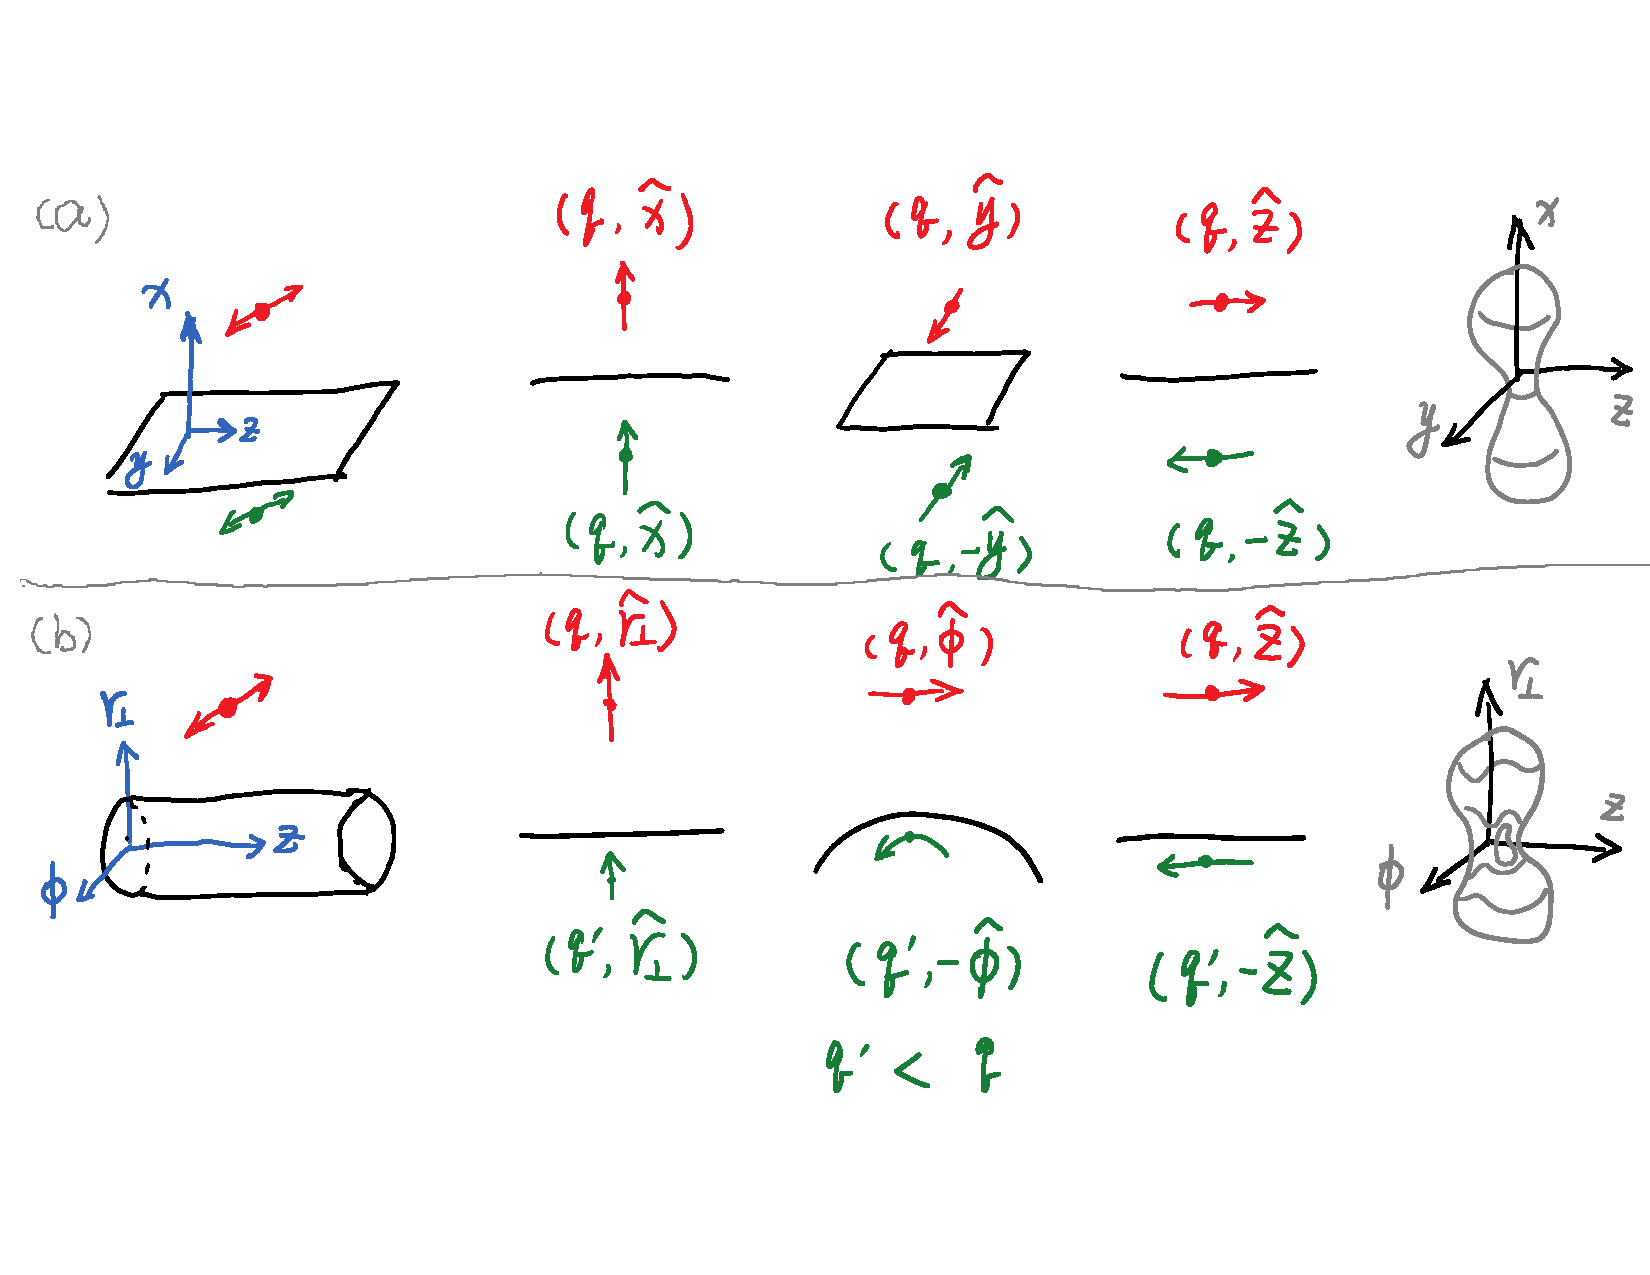
\includegraphics[width=0.8\textwidth]{../media/Figs/dipoleorientation}}
\caption[Modified dipole decay rates due to the interference of the radiations from the dipole and its image dipole mirrored on flat and cylindrical surfaces.]{Modified dipole decay rates due to the interference of radiations from the dipole and its image dipole mirrored on flat (a) and cylindrical (b) surfaces. Coordinate systems are defined on the left. 
We picture the dipole as an oscillator of two opposite charges separated by some distance. 
In the middle plots, the red arrows (on top of the reference interface lines) indicate the directions of dipole sources at a moment. The green arrows (below the interface) indicate the image dipole below the medium interface. 
We ignore the separation of charges in the dipole source and establish a qualitative physical intuition in thinking about how the dipole orientation affects the spontaneous emission rate of the dipole. 
Three orthogonal dipole orientations are considered. Emission surfaces are illustrated on the right. }\label{fig:dipoleinterferencepic}
\end{figure}

With a flat surface interface [Fig.~\ref{fig:dipoleinterferencepic} (a)], the dipole source has a mirror dipole with the same distance to the interface and the same oscillation strength as the source yet a mirrored oscillation direction in the static limit. Using three orthogonal dipole orientations, we find that, if the source dipole oscillates along the $ x $ direction perpendicular to the interface, the mirrored dipole has the same oscillation direction as the source and could contribute a constructive interference at the source dipole position when the source dipole is close to the interface. This could yield an enhanced spontaneous emission rate. To the extreme, when the dipole is placed on the surface, the emission rate will be enhanced twice as that of the free-space case. In contrast, if the source dipole is orientated along the $ y $ and $ z $ directions, the interference from the mirrored dipole will be destructive, which reduces the emission rate. As the dipole approaches the interface, all photon emissions will be canceled. Note that there is a degeneracy over the choice of $ y $ and $ z $ directions. In other words, $ y $ and $ z $ directions can be any two orthogonal directions parallel to the interface, and the emission rates on both directions will have the same amplitude.

Qualitatively, when we use a cylindrical waveguide as the medium interface [Fig.~\ref{fig:dipoleinterferencepic} (b)], the dipole mirroring will yield a smaller oscillation amplitude and shorter distance below the interface than the case if only the interface is changed to a flat surface (equivalent to make the radius of the cylinder to infinity). 
This property of curved interfaces makes the constructive and destructive interference between the dipole source and the image dipole less complete than the case of a flat interface. 
Particularly, the destructive interference when the dipole is orientated along the $ y $ axis--when the interface along $ y $ is curved--could be much weaker than along the $ z $ axis--when the interface along $ z $ can be treated as straight.
We plot out the emission surface of a dipole placed outside of a cylindrical waveguide with $ r'_\perp=a $ (dipole on the surface) and $ r'_\perp=2a $ in Fig.~\ref{fig:emissionsurfacenanofiber}. 
Using the cylindrical coordinate system, we find that the decay rate due to a $ z $-polarized dipole attains the minimum value while that of a $ r_\perp $-polarized dipole reaches the maximum, and the decay rate of a $ \phi $-polarized dipole is in the middle range. 
 
\begin{figure}[!tbp]
\centering\makebox[\textwidth]{
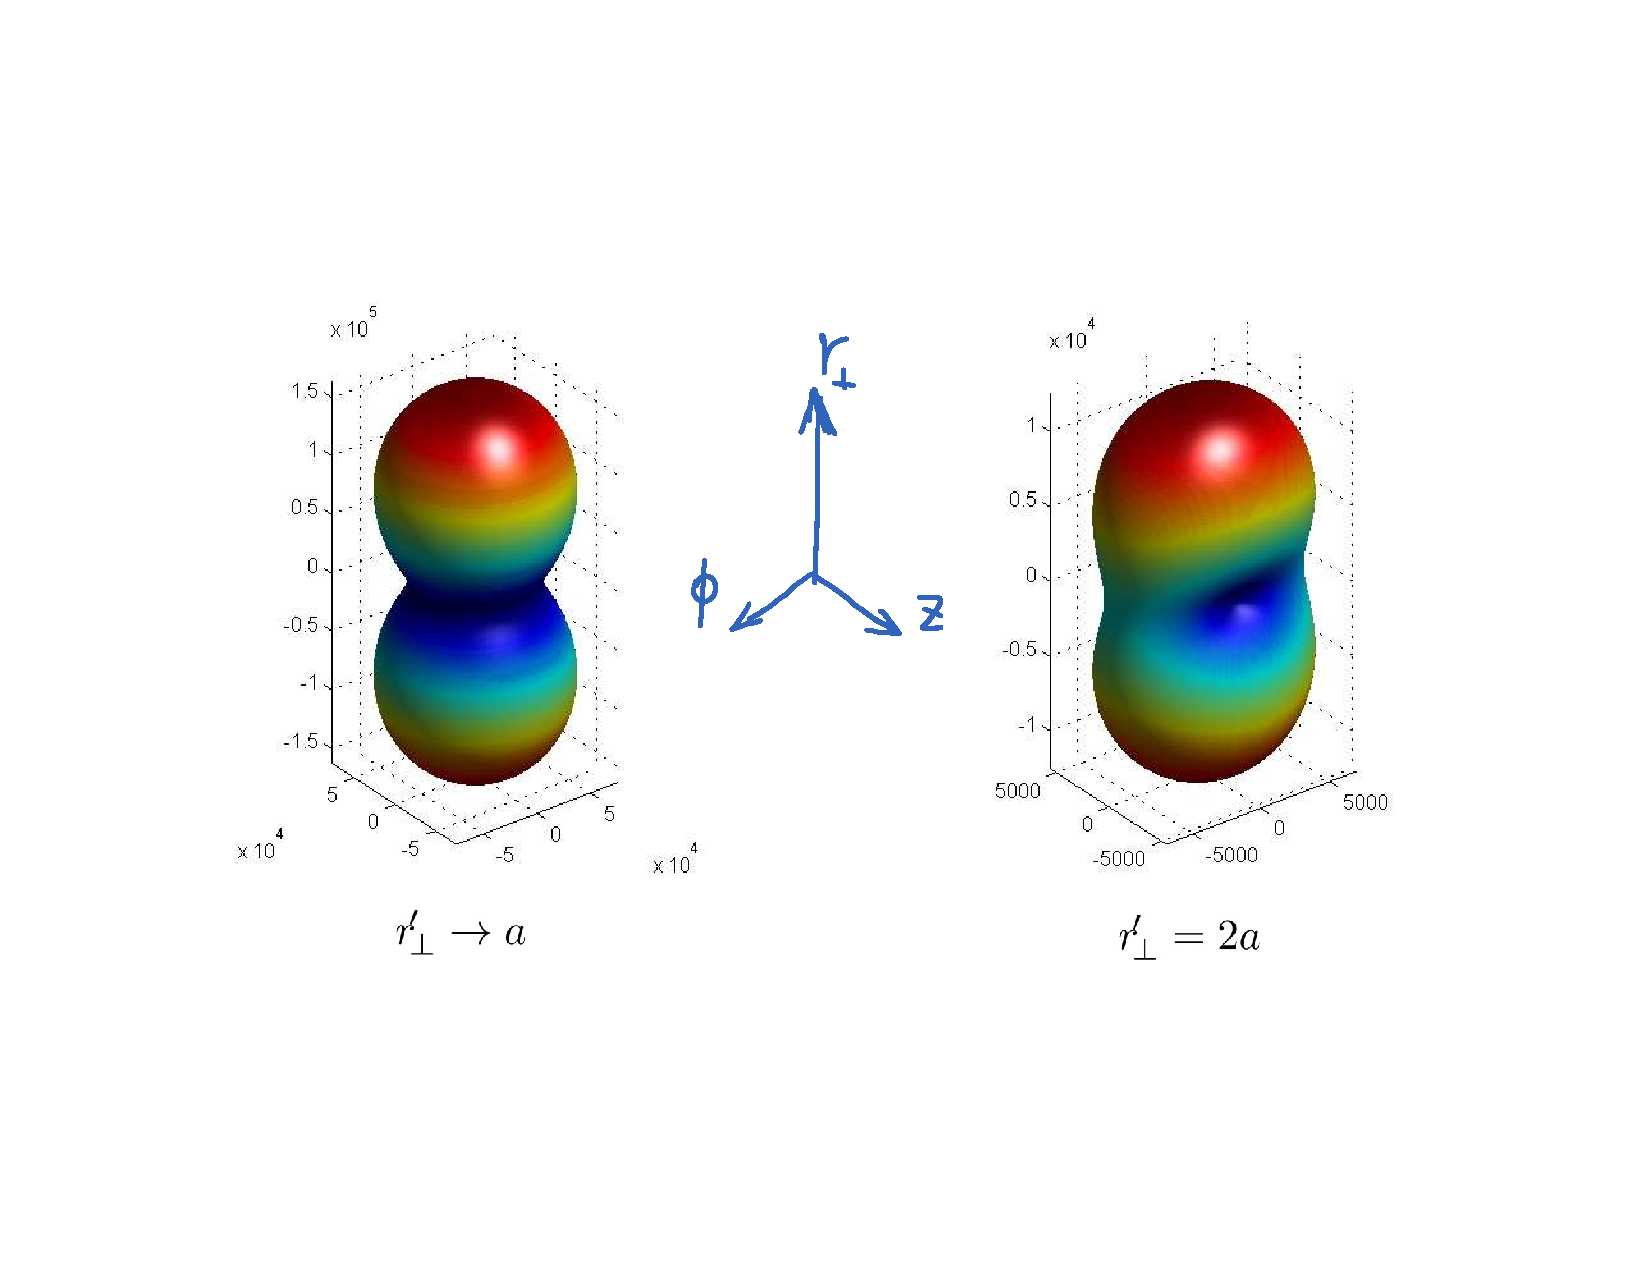
\includegraphics[width=0.8\textwidth]{../media/Figs/emissionsurfacefiber}}
\caption{Dipole emission surfaces of a dipole placed on the surface ($ r\!_\perp=a $) and outside ($ r\!_\perp=2a $) of a nanofiber.} \label{fig:emissionsurfacenanofiber}
\end{figure}

The range of $ \{\Gamma_1,\Gamma_2,\Gamma_3 \} $ characterizes the anisotropy of the medium interface for the modification of dipole emissions. 
From Fig.~\ref{fig:emissionsurfacenanofiber}, we can picture the emission surface of a dipole on top of a flat interface similar to the one in the nanofiber case with $ r'_\perp =a$. 
When the dipole is moving away from the flat surface, the contrast between $ \Gamma_y $ ($ \Gamma_z $) and $ \Gamma_x $ due to a dipole orientated along the $ y $ ($ z $) and $ x $ directions, respectively, will reduce gradually.
In general, the anisotropy of a flat medium interface is stronger than that of a curved interface. 
This is one intuitive guideline when we design a waveguide to enhance the anisotropic properties of waveguide-induced decay rates and phase shifts as we will discuss in Chapter`~\ref{chap:birefringence} and~\ref{chap:Faraday}. 

To find the equivalent dipole orientation of a given atomic state and probe, we first find out what the possible quantum transitions are from the initial atomic state under the polarization of the light, and then find out the branching ratios of the $ \sigma_\pm $ and $ \pi $ transitions following Eq.~\eqref{eq:dipolem'meq}, for example, where the correspondence between spherical quantum transitions and dipole orientations are determined by
\begin{align}
\sigma_+ &\leftrightarrow \mathbf{d}_+\propto \frac{1}{\sqrt{2}}(i\mathbf{e}_{r\!_\perp}+\mathbf{e}_\phi),\\
\pi &\leftrightarrow \mathbf{d}_0 \propto \mathbf{e}_z,\\
\sigma_- &\leftrightarrow \mathbf{d}_-\propto \frac{1}{\sqrt{2}}(-i\mathbf{e}_{r\!_\perp}+\mathbf{e}_\phi).
\end{align}
When the quantum transitions have different resonance frequencies, we group the physical processes by the corresponding frequencies and calculate the decay rates using the Green's tensors at the correct frequencies accordingly, and then sum them up to obtain the total decay rate for the system.
This method works obviously for atoms in pure states. In fact, this treatment also applies to mixed states. 
For example, we consider a completely mixed state, which has the equal possibility of generating $ \gamma_+ $, $ \sigma_- $ and $ \pi $ transitions. In terms of the dipole moment tensor, $ \tensor{\boldsymbol{\rho}} $, we have
\begin{align}
\tensor{\boldsymbol{\rho}} &=\frac{1}{3}(\tensor{\boldsymbol{\rho}}_++\tensor{\boldsymbol{\rho}}_0+\tensor{\boldsymbol{\rho}}_-)=\frac{d_0^2}{3}\unittensor.
\end{align}
The decay rate for such a case can be calculated by
\begin{align}
\Gamma &=\frac{2}{3\hbar}d_0^2 \mathrm{tr}\left\{ \mathrm{Im}[\GFT(\br',\br')] \right\}=\frac{1}{3}(\Gamma_1+\Gamma_2+\Gamma_3).
\end{align}
This is equivalent to assuming that the dipole is uniformly pointing in all directions, and hence
$\Gamma = \int \frac{\mathrm{\Omega}}{4\pi}\Gamma(\theta,\phi)=\frac{1}{3}(\Gamma_1+\Gamma_2+\Gamma_3)$ based on Eq.\eqref{eq:Gammathetaphi}.


This geometric perspective might be helpful to design nanophotonic waveguide interfaces and atomic states to enhance quantum tomography and control protocols.
For our study, we are interested in quantum measurements, which require us to generalize this idea to our context.

\subsection{Enhanced anisotropy of guided modes with different geometries of waveguides}
For the quantum measurement scenario we are interested in, only guided modes will be detected. Therefore, we define the decay rates coupled to a particular guided mode labeled by $ \mu $ with degeneracies of propagation directions and polarizations as
\begin{align}
\Gamma_\mu &= \frac{2}{\hbar}\left\{ \mathbf{d}\cdot \mathrm{Im}[\GFT_\mu(\br',\br')]\cdot \mathbf{d}^* \right\},
\end{align}
where 
\begin{align}
\GFT_\mu (\br',\br';\omega_{eg}) &= i\pi \frac{\omega_{eg}}{v_g}
		\mathbf{u}_\mu (\br_{\!\perp}^\prime)\mathbf{u}^*_\mu (\br_{\!\perp}^\prime) 
\end{align}
based on Eq.~\eqref{Eq::ImGreenLocal_general}. 
Since the phase shift of a guided mode after atom-light interaction is proportional to the coupled $ \Gamma_\mu $ [see Eq.~\eqref{phaseshiftGamma1D_nanofiber}], we can use the decay rates coupled to the two orthogonal modes of a mode basis to characterize the polarization transitions of the guided light. 
Therefore, the contrast of the decay rates coupled to two basis modes $ \mu_1 $ and $ \mu_2 $ defines the anisotropic property of the system. 
Using the $ H $ and $ V $ mode basis and assuming that the polarizability of the atom is scalar, $ \Gamma_H-\Gamma_V $ is maximized when the intensity difference between the $ H $ and $ V $ modes has the largest contrast, which is consistent with Eq.~\eqref{eq:birefringencerotang}. 
%defining the polarization transform from the first principle. 
In practice, one of our goals is to find a proper geometry so that the quantum measurement is enhanced due to the anisotropy of the waveguide modes. 
See Fig.~\ref{fig:anisotropybirefringence} for the example of a measurement geometry using the birefringence effect.

\begin{figure}[!tbp]
\centering\makebox[\textwidth]{
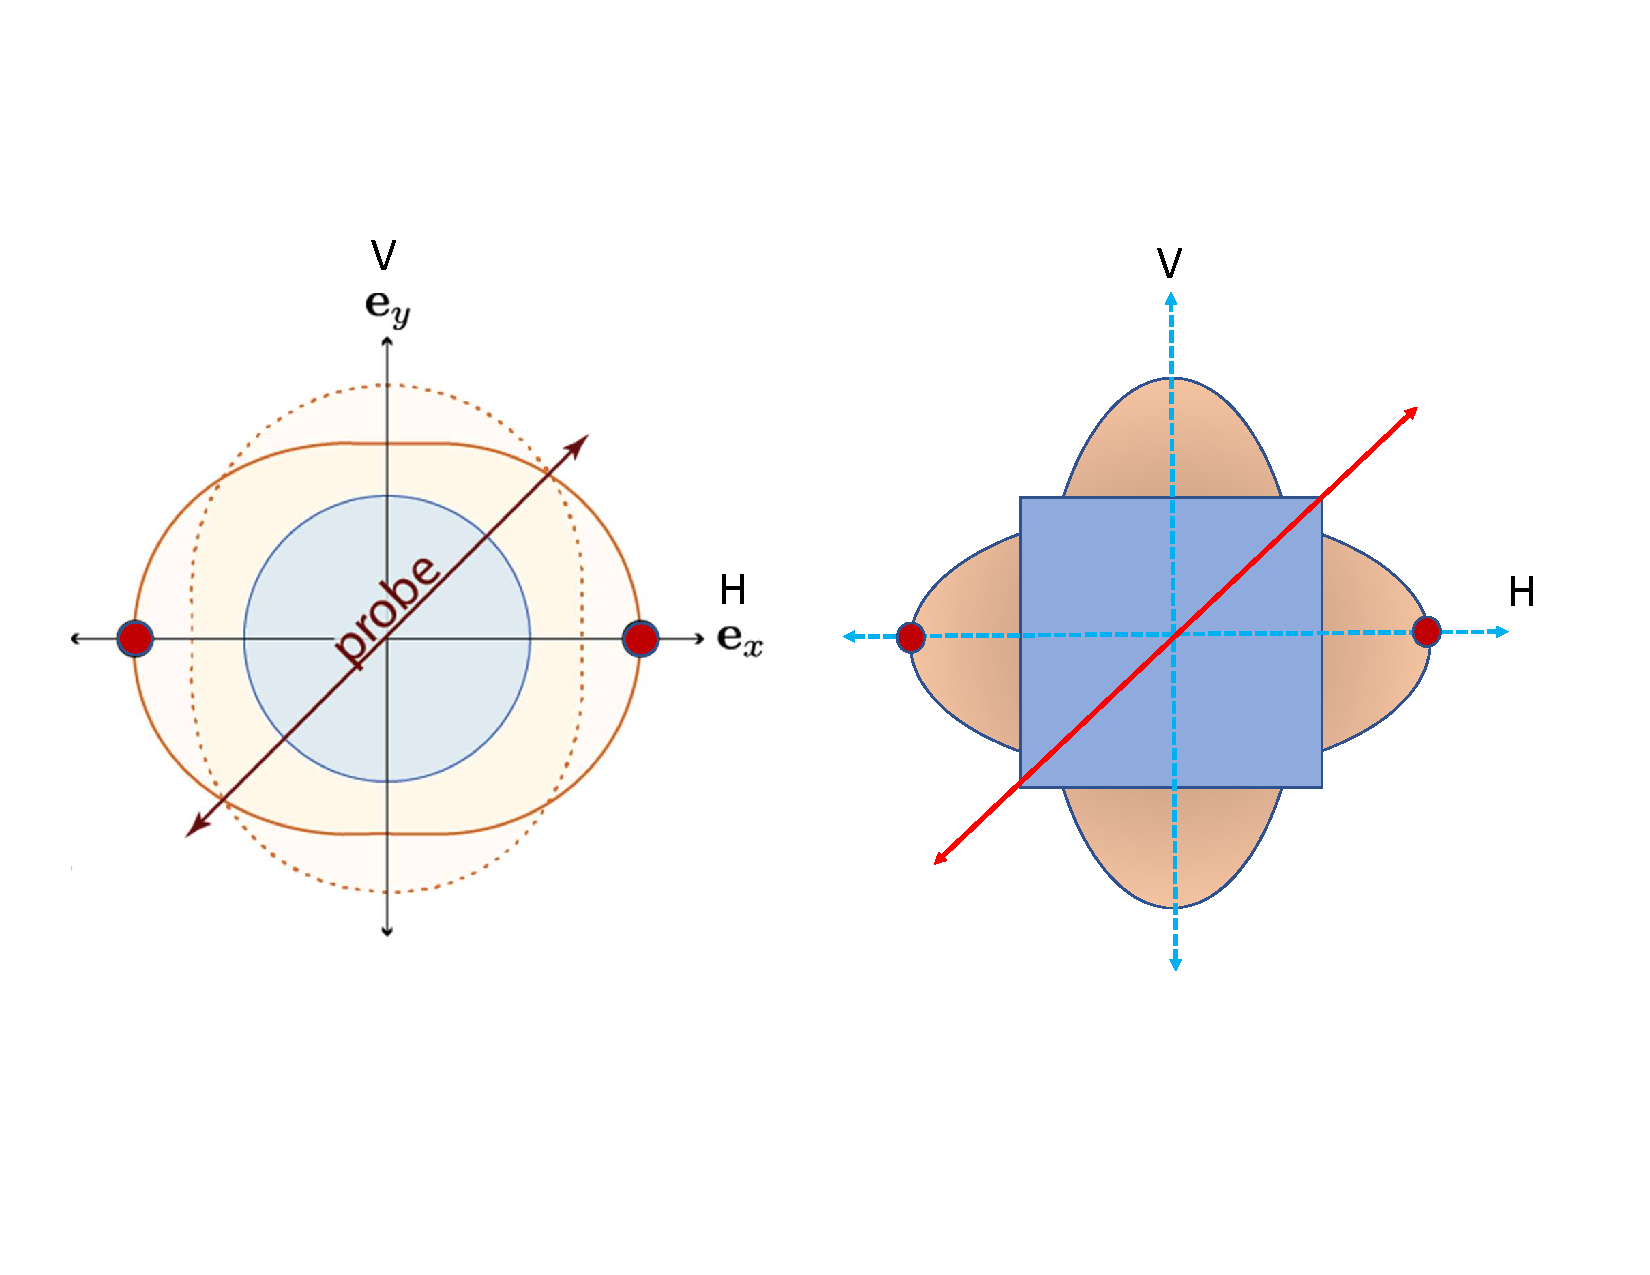
\includegraphics[width=0.8\textwidth]{../media/Figs/anisotropicmodes}}
\caption[Anisotropic guided modes and quantum measurement geometry for a nanofiber and a \SWG using the birefringence effect.]{Feasible quantum measurement geometry designs for a nanofiber (left) and a \SWG (right) using the birefringence effect by maximizing the anisotropy of local guided mode components. At the atom positions, the intensity difference between the $ H $ and $ V $ modes reaches the maximum value, which could be beneficial to enhance the birefringence rotation of the guided light even with a scalar polarizability of the atoms. }\label{fig:anisotropybirefringence}
\end{figure}

Based on a naive intuition that the confinement of light might be stronger for a waveguide with a square cross-section than a rounded one, a \SWG may have some advantages of enhancing the quantum measurement of some type over the nanofiber geometry. 
However, to fully understand the figure of merit of design and optimization, we have to consider the state space of the atoms and properties of the quantum measurement protocols. 
We will extend this discussion of protocol designs and optimizations in-depth in Chapters~\ref{chap:birefringence} and~\ref{chap:Faraday} using the concept of cooperativity, which is one of the cores of this dissertation.


%</emissionrates>
%###################################################################################
\bibliographystyle{../styles/abbrv-alpha-letters-links}
\bibliography{../refs/Archive,../chap5/Nanofiber}
%%%%%%%%%%%%%%%%%%%%%%%%%%%%%%%%%%%%%%%%%%%%%%%%%%%%%%%%%%%%%%%%%%%%%%%%%%%%%%%%%%%%%

\printindex
%\cleardoublepage
%\thispagestyle{plain}
%\phantomsection
%\printindex{ai}{Author Index}
%\chaptermark{Author Index}
%\thispagestyle{plain}
%\printindex{si}{Subject Index}
%\chaptermark{Subject Index}
\end{document}